\documentclass{report}
\usepackage{amsmath}
%\usepackage{amssymb} # it does not work with MnSymbol
\usepackage{amsthm,mathrsfs}
\usepackage{enumitem}
\usepackage[top=1in, bottom=1in, left=1in, right=1in]{geometry}
\usepackage{bm}
\usepackage{physics}
\usepackage{multirow}
\usepackage{tabularx}
\usepackage{graphicx}
\usepackage{hyperref}
\usepackage{enumitem}
\usepackage{booktabs}
\usepackage{cite}
\usepackage{algorithm}
\usepackage{algpseudocode}
\usepackage{cprotect}
\usepackage{graphicx}
\graphicspath{ {figures/} }
%Font used for low resolution printer, i.e 
\usepackage[no-math]{fontspec}
\usepackage{fourier}
\usepackage{MnSymbol}
\setmainfont{Linux Libertine O} 
%------------------------------
\author{Fang Wang}
\title{ \textbf{\huge{On the Equivalence of Tests for Outliers for Pareto and Exponential Distributions}}} 
\DeclareMathOperator{\se}{se}
\DeclareMathOperator{\bias}{bias}
\begin{document}
\newcommand{\RR}{\mathbb{R}}
\newcommand{\ZZ}{\mathbb{Z}}
\newcommand{\NN}{\mathbb{N}}
\newcommand{\QQ}{\mathbb{Q}}
\newcommand{\CC}{\mathbb{C}}
\newcommand{\e}{\mathrm{e}}
\newcommand{\sumi}[2][1]{\sum\limits_{i=#1}^{#2}}
\newcommand{\sumk}[2][1]{\sum\limits_{k=#1}^{#2}}
\newcommand{\sumj}[2][1]{\sum\limits_{j=#1}^{#2}}
\newcommand{\sumx}[2][1]{\sum\limits_{x=#1}^{#2}}
\newcommand{\sumn}[2][1]{\sum\limits_{n=#1}^{#2}}
\newcommand{\prodi}[2][1]{\prod\limits_{i=#1}^{#2}}
\newcommand{\prodk}[2][1]{\prod\limits_{k=#1}^{#2}}
\newcommand{\prodj}[2][1]{\prod\limits_{j=#1}^{#2}}
\newcommand{\E}[2][]{ \mathbb{E}_{#1} \left[ #2 \right]}
\newcommand{\Var}[1]{ \mathrm{Var} \left[ #1 \right]}
\newcommand{\Cov}[1]{ \mathrm{Cov} \left[ #1 \right]}
\renewcommand{\P}[2][]{ \mathbb{P}_{#1} \left( #2 \right)}
\newcommand{\iidis}{\stackrel{iid}{\sim}}
\newcommand{\toP}{\stackrel{P}{\to}}
\newcommand{\toD}{\stackrel{\mathrm{D}}{\to}}
\newcommand{\eqD}{\stackrel{\mathrm{D}}{=}}
\newcommand{\toas}{\stackrel{\mathrm{a.s}}{\to}}
\newcommand{\I}[1]{\mathbb 1_{\{#1\}}}
\newtheorem{thm}{Theorem}[chapter]
\newtheorem{prop}{Proposition}[chapter]
\newtheorem{lem}{Lemma}[chapter]
\newtheorem{cor}{Corollary}[chapter]

\theoremstyle{definition}
\newtheorem{defn}{Definition}[chapter]
\newtheorem{eg}{Example}[chapter]

\theoremstyle{remark}
\newtheorem*{rem}{Remark}

\maketitle

\begin{abstract}
    This thesis discusses the outlier detection problem with slippage alternative hypothesis for exponential and Pareto distributions. 
    We show that statistics used for testing slippage alternative hypothesis of exponential samples can be easily adapted to test for the Pareto case with the same critical values and power under certain regularity conditions. 
    The exact distributions of some specific statistics are derived, and their performance are examined through a Monte Carlo simulation study. 
    We observed that the classical Dixon statistic has the best performance in terms of power among all test statistics examined.
\end{abstract}

\section*{Acknowledgements}
First, I would like to thank my supervisor, Prof. Narayanaswamy Balakrishnan, for his supportive encouragement and
patient guidance throughout my time being his student. I really appreciate his crystal clear explanations and insightful comments 
he gave to me; without those, this thesis could not have been finished. 

I would also like to thank all  faculty members and staff in our department for their help in my life and study. In particular,
I want to thank Prof. Angelo Canty for teaching me many practical skills and useful advices on how to conduct research;
my previous work experience with him greatly helped me during this work.

Finally, my thanks go to my family for their love and encouragement throughout the years.



\tableofcontents

\chapter{Introduction} \label{chapter 1}

\section{Outliers and Outlier Detection Problem}

The outliers, in a sample of observations, is a subset of observations that appears to be inconsistent with the rest of the data and the assumption proposed
on the dataset \cite{grubbs1969procedures}. Outliers can arise in many ways, varing from a human recording error to the the natural inherent variability of
the data.

The problem of outlier detection is detecting  the outliers from a sample of observations and these have found many
 practical applications such as fraud detection \cite{ferdousi2006unsupervised} and
genetics \cite{norton2018outlier}. 

Whether an observation is an outlier depends on one’s subjective prior knowledge on the data
the observation is coming from; hence, the definition of an outlier is subjective. When an implausible observation arises, one may conclude a
misrecording happened and discard it, but such an observation may convey some important information about underline population; for example, it may
suggests a contamination of the data; that is, some of the observations do not come from the distribution that the data are assumed to have come from,
and this motivates the contamination model.


\subsection{Contamination Model and Slippage Alternative}


Suppose we have observations $(x_1\ldots,x_n)$ which are assumed to be independent and identically distributed (iid) samples of $(X_1,\ldots,X_n)$ and each $X_j$ has distribution $F$ under the null hypothesis $H_0$. 
If some of the observations $\{x_1,\ldots,x_r\}$ are unlikely coming from $F$, then one can conclude that $H_0$ is false, but there is more than one way to
construct the alternative hypothesis $\overline{H}$. We now formally define the null hypothesis as follows:

\begin{defn}[null hypothesis of contamination model] \label{defn: H_0}
    Let $x_1,\ldots,x_n$ be a sample of $n$ observations. Then under the null hypothesis $H_0$, $x_1,\ldots,x_n$ are observations of
    $X_1,\ldots,X_n$, where $X_1,\ldots,X_n$ are independent random variables with common distribution $F$.
\end{defn}

One possible $\overline{H}$ is $\overline H : X_j \sim G$ for all $X_j$, where $G$
is a distribution different from $F$ and this is known as the inherent alternative. One classical example of inherent alternative is
the hypothesis testing for one population mean, where $F$ and $G$ are usually same family of distributions but with different expectation.

One can also formalize $\overline H$ as the mixture distribution, so that $\overline H$ becomes $X_j \sim (1-\lambda)F + \lambda G$ where $\lambda$ is a
small positive real number. One should be cautious about the cyclic argument of the $\lambda$ being small, since $\lambda$ being small justifies
the outliers are rare but rare outliers also implies $\lambda$ being small. 

In this study, we will consider the alternative hypothesis known as the slippage alliterative constructed 
as follows: We assume that, expect for a small fixed number $r$ of observations, all arose
from $F$, but theses $r$ observations arose from a modified version of $F$, say $\overline F$. In this study, we will focus on the cases where $F$ and $\overline F$ are Pareto and exponential
distributions with different parameters, and we will use $H_r$ to denote the slippage alternative hypothesis, where $r$ of the $n$ observations came from $\overline F$.
We will restrict ourselves to the univariate case, and we can then formally define the slippage alternative hypothesis as follows:

\begin{defn}[slippage alternative of the contamination model] \label{defn: slippage Hr}
    Let $x_1,\ldots,x_n$ be a sample of $n$ observations with null hypothesis $x_1,\ldots,x_n$ that they are independently from a distribution $F$. Let
    $x_{(1)} < x_{(2)} <  \cdots < x_{(n)}$ be the order statistics of $x_1,\ldots,x_n$. Then under the slippage alternative $H_r$,
    the sample $x_{(1)},\ldots x_{(n-r)}$ are independent observations from distribution $F$ and $x_{(n-r+1)},\ldots, x_{(n)}$ are independent observations
    from distribution $\overline F$ with $F \neq \overline F$.
\end{defn}

As an illustrative example, we generated six sets of random samples of size $15$,
where for each random sample, $10$ of them came from exponential distribution with mean $1$ while other $5$ are contaminated coming 
 from exponential distribution with mean $2$; the discussion on the sample generation method are postponed to the Section \ref{sec: simulation methods}.
The random samples generated are depicted in Figure \ref{Figure: slippage sample},
where three sets of samples generated with slippage alternative assumption are plotted
in panel A and other three sets of samples without this assumption are given in the panel B.



\begin{figure}[hbtp]
    \centering
    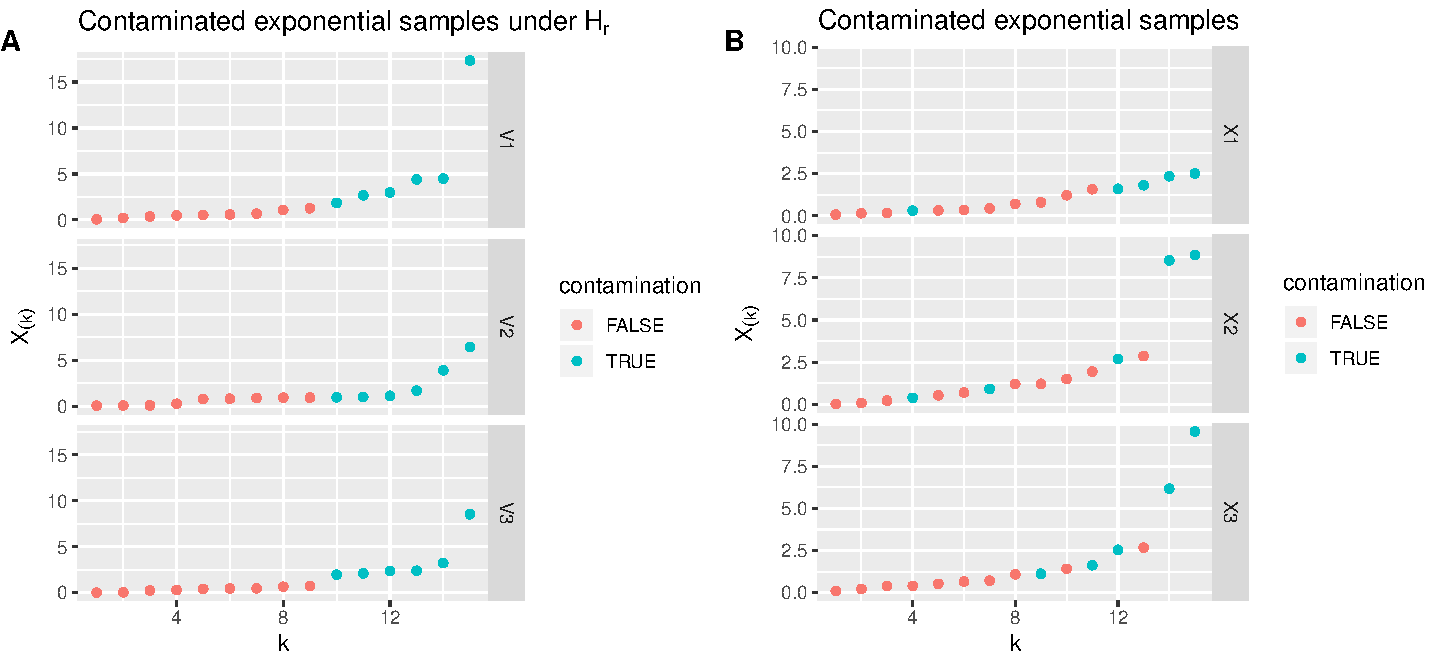
\includegraphics[scale = 0.6]{plot_0.pdf}
    \caption{Contaminated exponential random samples with $n =15, r =5, \E{F} =1, \E{\overline{F}} = 2$}
    {\label{Figure: slippage sample}
        \par {\small \begin{itemize}
            \item[A] Three random samples of exponential observations under slippage alternative\\
            \item[B] Three random samples of exponential observations with contamination but does not have assumption of slippage alternative.
        \end{itemize}
    }}
\end{figure}

Hereafter, we will use capital letter $X_1,\ldots,X_n$ to denote the random variables, $X_{(1)},\ldots. X_{(n)}$ to denote the order statistics of $X_1,\ldots,X_n$,
lower case letter $x_1,\ldots,x_n$ to denote the sample of $X_1,\ldots X_n$ and lower case $\mathbf x = (x_1,\ldots, x_n)$ denoted the vector of observations. 

\subsection{Discordancy Test}
The hypothesis testing procedures that test for outliers are known as discordancy tests. There are two major tests against $H_0$ defined in
Definition \ref{defn: H_0}, and they are sequential tests and block tests \cite{barnett1984outliers}. A sequential test for the outlier detection detects the outliers by applying the
statistic test repeatedly, starting with the most extreme sample observation; if we reject $H_0$, then apply the test to the sample with
the most extreme sample removed, and so the procedure is stopped once we fail to reject $H_0$ \cite{rosner1975detection}.

The block test is simpler, where the number of possible contamination sample $r$ is specified and the hypothesis testing is done with
a single test. The block tests suffer from the problem of swamping and masking, when the
number of hypothesized outliers is different from the actual number of outliers, but this is not a problem under slippage alternative. Because block tests are easy to
interpret, we restrict ourselves to the case of slippage alternative in our study.

\section{Organization of the Thesis}
The rest of this report is organized as follows: A review of mathematical results that will be used
to establish the distribution of test statistics proposed by Zerbet and Nikulin\cite{zerbet2003new} and
Jabbari Nooghabi\cite{jabbari2019detecting} and an introduction of simulation methods used is given in Chapter \ref{chapt: Methods}. The exact distributions of test statistics given by Jabbari Nooghabi and Zerbet and Nikulin, under $H_r$,
are given in Chapter \ref{chapt: Discordancy Tests}. Results of a simulation study and the conclusions drawn are presented in Chapter \ref{chapt: Simulation Study}.


\chapter{Methods} \label{chapt: Methods}

In this thesis we derive the distribution of $Z_r$ given by
Zerbet and Nikulin\cite{zerbet2003new} and $\tilde R_r$ given by Jabbari Nooghabi \cite{jabbari2019detecting} under $H_r$, 
forwhich we need some key distributional results that are presented in Section \ref{sec: mathematical result}. 

Then, we characterize the distribution of order statistics after
monotone transformation assuming some regularity conditions in Section \ref{sec: monton trans}. In particular, Corollary \ref{cor: distribution of log Pareto OS under Hr}
plays a key role in deriving the correct distribution of test statistic $\tilde Z_r$ introduced in \cite{jabbari2019detecting}, and justify
the equivalence of some test statistics we investigate.

To verify the theoretical results derived and also to observe some other characteristic of the test statistics we study here,
we conduct the simulation studies, and the algorithms and some other facts are summarized in Section \ref{sec: simulation methods}.


\section{Mathematical Results} \label{sec: mathematical result}

The follwing lemma will be used in the derivation of the distribution of tests $Z_r$ and $R_r$ to simplify and rewrite the expressions.

 \begin{lem}\label{Lemma: partial fraction}
     Let $\{a_k\}_{k=1}^m$ be a finite number of distinct real number and $x \in \CC$. Then
     \[ 
         \prodk[1]{m} \frac{1}{x - a_k} = \sumn[1]{m} \frac{1}{x-a_n} \prod_{\substack{i = 1, i\neq n}}^{m} \frac{1}{a_n -a_i}.
     \]
 \end{lem}
 
 \begin{proof}
     We will prove the result by induction on $k$. The case for $k =1$ clearly holds. Case for $k =2$
     also holds, since
     \[ 
         \frac{1}{(x-a_1)(x-a_2)} = \frac{1}{(x-a_1)(a_1 - a_2)} + \frac{1}{(x-a_2)(a_2 - a_1)}.
     \]
     Now assume the case holds for $k = m-1$ and consider the case for $k =m$. Because
 
     \begin{align*}
         \prodk[1]{m} \frac{1}{x - a_k} &= \frac{1}{x - a_m} \prodk[1]{m-1} \frac{1}{x - a_k}
         \\
         &= \frac{1}{x - a_m} \sumn[1]{m-1} \frac{1}{x-a_n} \prod_{\substack{i = 1, i\neq n}}^{m-1} \frac{1}{a_n -a_i} &&\text{(by induction hypothesis)}
         \\
         &= \sumn[1]{m-1} \left( \frac{1}{a_n - a_m} \frac{1}{x -a_n} + \frac{1}{x-a_m}\frac{1}{a_m - a_n}\right) \prod_{\substack{i = 1, i\neq n}}^{m-1} \frac{1}{a_n -a_i}
         \\
         &= \left[\sumn[1]{m-1} \frac{1}{x-a_n} \prod_{\substack{i = 1, i\neq n}}^{m} \frac{1}{a_n -a_i}\right] + \sumn[1]{m-1} \frac{1}{x-a_m} \frac{1}{a_m - a_n} \prod_{\substack{i = 1, i\neq n}}^{m-1} \frac{1}{a_n -a_i}
         \\
         &= \left[\sumn[1]{m-1} \frac{1}{x-a_n} \prod_{\substack{i = 1, i\neq n}}^{m} \frac{1}{a_n -a_i}\right] + \frac{1}{x-a_m}\sumn[1]{m-1}  \frac{1}{a_m - a_n} \prod_{\substack{i = 1, i\neq n}}^{m-1} \frac{1}{a_n -a_i},
     \end{align*}
 
 where by induction hypothesis with $x = a_m$ that
 \begin{align*}
     \sumn[1]{m-1}  \frac{1}{a_m - a_n} \prod_{\substack{i = 1, i\neq n}}^{m-1} \frac{1}{a_n -a_i} &= \prodk[1]{m-1} \frac{1}{a_m - a_k}
     \\
     &= \prod_{\substack{i = 1, i\neq m}}^{m} \frac{1}{a_m -a_i},
 \end{align*}
 
 and therefore
 \begin{align*}
     \prodk[1]{m} \frac{1}{x - a_k} &=  \left[\sumn[1]{m-1} \frac{1}{x-a_n} \prod_{\substack{i = 1, i\neq n}}^{m} \frac{1}{a_n -a_i}\right] + \frac{1}{x-a_m}\prod_{\substack{i = 1, i\neq m}}^{m} \frac{1}{a_m -a_i}
     \\
     &= \sumn[1]{m} \frac{1}{x-a_n} \prod_{\substack{i = 1, i\neq n}}^{m} \frac{1}{a_n -a_i}.
 \end{align*}
 This proves the lemma.
 \end{proof}
 
The major tool used for deriving the distribution of $Z_r$ is characteristic function and the following result allows one
to obtain the pdf of the distribution of a continuous random variable from its characteristic function.

 \begin{lem}[Inversion Formula \cite{balakrishnan2004primer}] \label{Lemma : inversion formula}
     Let $X$ be  a continuous random variable with characteristic function $f(x)$ such that
     \[ 
         \int_{-\infty}^{\infty} \abs{f(x)} \dd{x} < \infty.
     \]
     Then, the pdf of $X$, $p(x)$, is given by
     \[ 
     p(x) = \frac{1}{2\pi} \int_{-\infty}^{\infty} e^{-itx} f(t) \dd{t}.
     \]
 \end{lem}

 \begin{lem} \label{Lemma: integration identity.}
     Let $b$ and $\theta$ be real numbers and $\theta  \neq 0$. Then,
     \[ 
         \int_0^\infty \frac{e^{-iwz}}{(b/\theta - iz)^r} \dd{z} = \frac{2\pi w^{r-1}}{(r-1)!} e^{-wb/\theta}.
     \]
 \end{lem}
 
 \begin{proof}
     Let $X$ be a random variable with $\mathrm{Gamma}(r,\theta/b)$ distribution. Then, the pdf $p(x)$ and characteristic function $f(x)$ of $X$ are given by
     \[ 
         p(x) =  \frac{w^{r-1}e^{-w/b}}{\Gamma(r) (\theta/b)^r },\quad x>0, \qquad \text{and} \qquad f(x) = (1-ix \theta/b)^{-r}.
     \]
     Then, it follows from Lemma \ref{Lemma : inversion formula} that
     \begin{align*}
        &&  2\pi p(w) &= \int_{-\infty}^{\infty} e^{-izw} f(t) \dd{z}
         & \\
        \iff&& 2\pi \frac{w^{r-1}e^{-w\theta/b}}{(\theta/b)^r(r-1)!} &= \int_0^\infty \frac{e^{-iwz}}{(1-iz\theta/b)^r} \dd{z}
         & \\
        \iff&& 2\pi \frac{w^{r-1}e^{-w\theta/b}}{(r-1)!} &= \int_0^\infty \frac{e^{-iwz}}{(b/\theta)^r  (1-iz\theta/b)^r} \dd{z}
         & \\
       \iff&& 2\pi \frac{w^{r-1}e^{-w\theta/b}}{(r-1)!} &= \int_0^\infty \frac{e^{-iwz}}{(b/\theta - iz)^r} \dd{z}   
     \end{align*}
     which proves Lemma \ref{Lemma: integration identity.}.
 \end{proof}
 
 The following lemma, was introduced by Chikkagoudar \textit{et al.} \cite{chikkagoudar1983distributions}, allows one to transform the problem of finding the distribution of order statistics into finding the distribution
 of independent exponential random variables. Since the characteristic function of sum of random variables is the product of the characteristic function
 of each summand only if the random variables summed up are independent, the following lemma is of critical importance. Prior to introducing
 the lemma, we first fix the notation and definition of the exponential distribution in the following definition.

 \begin{defn}[Exponential distribution]
     A random variable $X$ follows exponential distribution with mean parameter $\theta > 0$ if it has pdf of
     \[ 
         f(x) = \frac{1}{\theta} e^{-x/\theta}, \quad x >0
     \]
     and we denoted it by $X \sim \mathrm{Exp}(\theta)$.
 \end{defn}


 \begin{lem} \label{Lemma: order statistic transformation}
     Let $X_1, \ldots, X_{n}$ be independent $\mathrm{Exp}(\theta)$ random variables, 
      $X_{(1)},\ldots X_{(n)}$ be the order statistics of $X_1,\ldots,X_n$, and $Y_j = X_{(j)} - X_{(j-1)}$. Assuming the
      slippage alternative $H_r$, we then have
 
 \begin{align*}
     &X_{(1)},X_{(2)},\ldots,X_{(n-r)} \text{derived from $\mathrm{Exp}(\theta)$};
     \\
      & X_{(n-r+1)},X_{(n-r+2)},\ldots,X_{(n)} \text{derived from $\mathrm{Exp}(\theta/b)$,} \\
     &\quad \text{$0 < b \leqslant 1$, $b$ is unknown.}
 \end{align*}
      
      Then, $Y_j \sim \mathrm{Exp}(\theta(rb + n-r-j+1))$ for $ 1 \leqslant j \leqslant n-r$; 
      $Y_{n-r+j} \sim \mathrm{Exp}((\theta/b)(r-j+1)^{-1})$ for $ 1 \leqslant j \leqslant r$.
 \end{lem}
 
 \begin{proof}
 
     Let $\{N_t^k\}_{t\geq 0}$ be independent Poisson counting process with state space $\{0,1\}$, rate $1/\theta$ for $k\in\{1,\ldots,n-r\}$ and rate $\theta/b$ for $k \in \{n-r+1,\ldots n\}$. 
     Then, each $X_k$ is the sojourn time of $N_t^k$ in the stage $0$. Let
      \[ 
          N_t = \sumk{n} N_t^k,
      \]
     then $N_t$ is a Poisson process with state space $\{0,1,\ldots,n\}$. Assuming $X_{(0)} = 0$, then $Y_i = X_{(i)} - X_{(i-1)}$ is the sojourn time of $N_t$ in state $i-1$; that is,
     \begin{align*}
         \P{Y_i > t} &= \P{N_t < i \mid N_t = i-1 }
         \\
         &=\P{ \sumk[i]{n} N_t^k - \sumk[i]{n} - N_0^k = 0 }
         \\
         &= \P{ \sumk[i]{n} N_t^k- N_0^k = 0 }
         \\
         & = \prodk[i]{n} \P{N_t^k- N_0^k = 0}.
     \end{align*}
     If we assume $i \in \{1,\ldots,n-r\}$, then
     \begin{align*}
         \P{Y_i >t} &= \left[\prodk[n-r]{n} \P{N_t^k- N_0^k = 0}\right] \left[ \prodk[i]{n-r} \P{N_t^k- N_0^k = 0} \right]
         \\
         &= \left[\prodk[n-r]{n} \exp{ - \frac{b}{\theta} t }\right] \left[ \prodk[i]{n-r} \exp{- \frac{t}{\theta}} \right]
         \\
         &= \exp{ - \frac{rb}{\theta} t - \frac{n-r+1-i}{\theta} t}
     \end{align*}
     and $Y_i \sim \mathrm{Exp}( \theta(rb + n-r-i+1))$ as desired. If $i = n-r + j$ for $j \in \{1,\ldots,r\}$ then
     \begin{align*}
         \P{Y_{n-r+j} >t} &= \prodk[n-r+j]{n} \P{N_t^k- N_0^k = 0}
         \\
         &= \exp{ - (r+j+1)\frac{b}{\theta}t},
     \end{align*}
     and $Y_j \sim \mathrm{Exp}((\theta/b)(r-j+1)^{-1})$ for $ 1 \leqslant j \leqslant r$ as desired.    
 \end{proof}


\section{Distribution of Order Statistics Under Monotone Transformation} \label{sec: monton trans}

The goal of this section is to establish the main result that shows certain tests statistics used for testing $H_r$ for the exponential samples
can be easily adapted to test $H_r$ for the Pareto samples and the transformed test will have the same power and critical values.

\begin{thm} \label{thm: monoton transform of order stats}
    Let $X_1,X_2,\ldots, X_n$ be continuous random variables with density $f_1,\ldots, f_n$, respectively, where $f_i$ has the same support $(a,b)$ with $-\infty \leqslant a < b \leqslant \infty$. Let
    $g_1,\ldots,g_n$ be a collection of strictly increasing differentiable functions with domain $(a,b)$ and range $(c,d) \subseteq \RR$.
     Define random variable $Y_i = g_i(X_{(i)}),$ for $i =1,\ldots,n$.
    Then, the joint pdf of $Y_1,\ldots Y_n$ is given by
    
    \[ 
        f_{Y_1,\ldots,Y_n}(y_1,\ldots, y_n) = \begin{cases}
            n!\prodi{n} \abs{ \dv{g_i^{-1}}{y}}  f_i(y_i), & c < y_1 < y_2 <\cdots < y_n < d
            \\
            0, & \text{elsewhere.}
        \end{cases}
    \]
    \end{thm}
    
    \begin{proof}
        Since each $g_i$ is monotone increasing and $X_{(1)} < \cdots < X_{(n)}$, evidently the support of 
         of $Y_1,\ldots,Y_n$ is given by $\mathcal Y = \{(y_1,\ldots,y_n) : c < y_1 <\cdots < y_n < d \}$, which is the image of 
        the map $T: (x_1,\ldots, x_n) \mapsto (g_1(x_1),\ldots, g_n(x_n))$ from the
        set $\mathcal X_0 = \{a < x_1 < \cdots < x_n <b\}$. In fact, since each $g_i$ is an order preserving bijection,$T$ is
        a bijection from set $\mathcal X_{\sigma} =\{(x_{\sigma(1)},\ldots, x_{\sigma(n)}):(x_{\sigma(1)} < \cdots < x_{\sigma(n)} \}$ to $\mathcal Y$, where $\sigma$ is any
        permutation of the set $\{1,\ldots,n\}$.
    
         Consider the transformation of $T$ restricted on $\mathcal X_0$, which is given by
        $y_1 \mapsto g_1(x_1),\ldots, x_n \mapsto g_n(x_n)$. Then, Jacobian for $T^{-1}_{\mathcal X_0}$ is given by
    
        \[ 
             \abs{J_0} = \mathrm{abs}\left(\begin{vmatrix}
                \dv{g_1^{-1}}{y_1} & 0 &  \cdots & 0 \\
                0 & \dv{g_2^{-1}}{y_2} & \cdots & 0 & \\
                \vdots & \vdots & \ddots & \vdots \\
                0 & 0  & \cdots & \dv{g_n^{-1}}{y_n}
            \end{vmatrix}\right),
        \]
        which is equal to $\prodi{n} \abs{ \dv{g_i^{-1}}{y}}$. Since for any permutation $\sigma$, the Jacobian of $T^{-1}|_{\mathcal X_\sigma}$ can be obtained by interchanging the row of $J_0$,
        it differs from $J_0$ at most by a sign. 
    
        Let $S_n$ denotes all permutations on $\{1,\ldots,n\}$, and $J_\sigma$ denotes the Jacobian of $T^{-1}_{\mathcal X_\sigma}$.
        Because $\{\mathcal X_\sigma\}_{\sigma \in S_n}$ are mutually disjoint and partition the support of $X_1,\ldots,X_n$, 
        the pdf of $(Y_1,\ldots, Y_n)$ is given by
    
        \begin{align*}
            f_{Y_1,\ldots,Y_n}(y_1,\ldots, y_n) &= \sum_{\sigma \in S_n} \abs{J_{\sigma}} f(y_1,\ldots, y_n)
            \\
            &= \begin{cases}
                n! \prodk{n} \abs{ \dv{g_i^{-1}}{y}} f_i(y_i), & g(a) < y_1 < y_2 <\cdots < y_n < g(b)
                \\
                0, & \text{elsewhere,}
            \end{cases}
        \end{align*}
        where $n!$ comes from $S_n$ having $n!$ elements and the product of $f_i$ follows from the assumption $X_i$ are independent.
    \end{proof}

\begin{rem}
  This result is motivated by the classical proof for the distribution of order statistics. Here, we consider the case when $g_i$ are strictly increasing,
  one can also show that a similar result holds if $g_i$ are strictly decreasing functions.   
\end{rem}

By taking $g_i$ to be the identity map and $f_i$ to be the same density $f$ in the previous theorem, we obtain the follwing well known fact.

\begin{cor} \label{cor: distribution of order stats}
    Let $X_1,X_2,\ldots, X_n$ denote a random sample from a distribution of the continuous
type having a pdf $f(x)$ that has support $(a,b)$ with $-\infty \leqslant a < b \leqslant \infty$. Let $Y_k = X_{(k)}$ for
$k = 1,\ldots,n$, then
then the joint pdf of $Y_1,\ldots Y_n$ is given by

\[ 
    f_{Y_1,\ldots,Y_n}(y_1,\ldots, y_n), = \begin{cases}
        n! f(y_1) f(y_2) \cdots f(y_n), & 0 < y_1 < y_2 <\cdots < y_n < b
        \\
        0, & \text{elsewhere.}
    \end{cases}
\]
\end{cor}

Now we shall prove Corollary \ref{cor: distribution of log Pareto OS under Hr},
which connects the order statistics of exponential samples and Pareto samples. For this purpose, we
first introduce the definition of Pareto distribution.
\begin{defn}[Pareto distribution]
    A random variable $X$ follows $\mathrm{Pareto}(\alpha,\theta)$ distribution if its pdf is given by
    \[ 
        f(x;\alpha,\theta) = \frac{\alpha \theta^{\alpha}}{x^{\alpha +1}} I_{\{ x \geqslant \theta >0\}},
    \]
    where $\theta$ and $\alpha$ are both positive parameters.
\end{defn}

We note that a Pareto random variable can be transformed into an exponential random variable
as shown in the following lemma, and it makes the result given in Corollary \ref{cor: distribution of log Pareto OS under Hr} very intuitive.

\begin{lem} \label{lem: log of Pareto is exp}
    Suppose $X \sim \mathrm{Pareto}(\alpha,\theta)$ and $Y = \log(X/\theta)$. Then, $Y \sim \mathrm{Exp}(\alpha)$.
\end{lem}

\begin{proof}
    Let $f_X$ and $f_Y$ be the pdf of $X$ and $Y$, respectively. Then, we have
    \[ 
        f(x) = \alpha \theta^\alpha x^{-(\alpha+1)}
    \]
        for $x\geqslant 0$. Since the function $g : x \mapsto \log(x/\theta)$ is a bijection
        on the support of $X$ with inverse $g^{-1} : y \mapsto \theta e^y$, the pdf of $Y$
        is given by
        \begin{align*}
            f_Y(y) &= f_X(g^{-1}(y)) \abs{ \dv{g^{-1}}{y}}
            \\
            &= \alpha \theta^{\alpha}[\theta e^y]^{-(\alpha +1)} \abs{\theta e^{y}}
            \\
            &=\alpha e^{-\alpha y},
        \end{align*}
        which is the pdf of $\mathrm{Exp}(\alpha)$ random variable and the Lemma is thus proved.
    \end{proof}

Because the logarithm function is a monotone transformation, one would expect an analogous result
of the Lemma \ref{lem: log of Pareto is exp} holds for order statistics from Pareto
 and exponential distributions, as shown in the Corollary below.

\begin{cor} \label{cor: distribution of log Pareto OS}
    Let $X_1, \ldots X_n$ and $E_1,\ldots, E_n$ be independent random variables with $ X_k \sim \mathrm{Pareto}(\alpha_k,\theta_k)$ and
    $E_k \sim \mathrm{Exp}(\alpha_k)$ for $k =1,\ldots,n$. Let $Y_k = E_{(k)}$ and $U_k = \ln(X_{(k)}/\theta_k)$, for $k =1,\ldots,n$.
    Then the random vector $\mathbf U =(U_1,\ldots, U_n)$ has the same distribution as $\mathbf Y = (Y_1,\ldots,Y_n)$.
\end{cor}

\begin{proof}
    Because each $X_k$ is independent and the function $g_k(y) = \ln(y/\theta_k)$ is differentiable and strictly increasing on $[0,\infty)$ with range same as its domain,
    we can apply Theorem \ref{thm: monoton transform of order stats} to obtain the pdf of $\mathbf U$. It follows from the definition that
    the support of $\mathbf U$ and $\mathbf Y$ are both $\mathcal U = \{(u_1,\ldots,u_n): 0 < u_1 < \cdots < u_n < \infty\}$. Let $f_k$ and $h_k$
    be the pdfs of $X_k$ and $Y_k$, respectively. Then for any $(u_1,\ldots,u_n) \in \mathcal U$, we have
    \begin{align*}
        f_{U_1,\ldots,U_n}(u_1,\ldots,u_n) &=  n! \prodk{n} \abs{ \dv{g_k^{-1}}{y}} f_k(y_k)
        \\
        &= n! \prodk{n} \alpha_k \theta_k^{\alpha_k}[\theta_k e^u_k]^{-(\alpha_k +1)} \abs{\theta_k e^{u_k}}
        \\
        &= n! \prodk{n} \alpha_k e^{-\alpha u_k} 
        \\
        &= n! \prodk{n} h_k(u_k).
    \end{align*}
 Then, it follows from Theorem \ref{thm: monoton transform of order stats}, with $g_i$ being the identity map, we verify that this is indeed the pdf of $\mathbf U$
 and the result follows.
\end{proof}

As another application of the previous corollary, we give an analogous result under $H_r$, which is the main result of this section.

\begin{cor} \label{cor: distribution of log Pareto OS under Hr}
    Let $X_1,\ldots, X_n$ be independent random variables with $X_1,\ldots,X_{n-r} \sim \mathrm{Pareto}(\alpha_1, \theta)$ and
    $X_{n-r+1},\ldots, X_{n} \sim \mathrm{Pareto}(\alpha_2,\theta)$. Let $E_1,\ldots, E_n$ be independent random variables with $E_1,\ldots,E_{n-r} \sim \mathrm{Exp}(\alpha_1)$ and
    $E_{n-r+1},\ldots, E_{n} \sim \mathrm{Exp}(\alpha_2)$. Let $Y_k = E_{(k)}$ and $U_k = \ln(X_{(k)}/\theta)$, for $k =1,\ldots,n$.
    Then the random vector $\mathbf U =(U_1,\ldots, U_n)$ has the same distribution as $\mathbf Y = (Y_1,\ldots,Y_n)$ under the slippage alternative $H_r$.
\end{cor}

\begin{proof}
    Because $\ln(X_k/\theta)$ has the distribution of $\mathrm{Exp}(\alpha_k)$, it is evident
    that the random vector $(\ln(X_1/\theta),\ldots, \ln(X_n/\theta))$ has the same distribution as $(E_1,\ldots, E_n)$. Then,
    it direct follows from the previous corollary that
    \begin{align*}
        \P{U_k \leqslant u \mid H_r} &= \P{\ln(X_{(k)}/\theta) \leqslant u \mid \max\{ \ln(X_{1}/\theta),\ldots, \ln(X_{n-r}/\theta)\} < \min\{\ln(X_{n-r+1}),\ldots,\ln(X_{n})\}}
        \\
        &= \P{Y_k \leqslant u \mid \max\{E_{1},\ldots,E_{n-r}\} < \min\{E_{n-r+1},\ldots,E_{n}\}}
        \\
        &= \P{Y_k \leqslant u \mid H_r}.
    \end{align*}
\end{proof}

\section{Simulation Methods} \label{sec: simulation methods}

Monte Carlo methods are experiments that make use of simulated random samples to estimate functionals of statistical densities and we now introduce some methods
that will be used.

\subsection{Slippage Random Sample Generation}


\subsubsection{Sample Generation Algorithm\ref{algorithm: Exp Hr sample}}

To conduct simulation studies and investigate the performance of statistical tests under slippage alternative $H_r$ defined in Definition \ref{defn: slippage Hr},
we need methods that generates random samples under $H_r$. Our study focuses on the case when $F$ and $\overline F$ are exponential or Pareto distributions,
but we only need to consider generating samples from exponential case, since it follows from Corollary \ref{cor: distribution of log Pareto OS under Hr}
that we can obtain random samples from Pareto distribution under slippage alternative by applying appropriate transformation on the exponential sample obtained.

\begin{algorithm}
    \caption{Algorithm for Generating Exponential Random Samples Under $H_r$} \label{algorithm: Exp Hr sample}
    \hspace*{0.02in} {\bf Input:} \\
     sample size : $n$ \\
     number of contaminated sample: $r$ \\
     the parameter for contaminated sample : $b, \theta$, where $b \in (0,1), \theta > 0$. \\
     \hspace*{0.02in} {\bf Output:}
       A sample $\mathbf X = (x_1,\ldots,x_n)$ under $H_r$.
       \begin{algorithmic}[1]
        \Repeat
          \State generating sample $\mathbf x = (x_1,\ldots,x_{n-r}) \iidis \mathrm{Exp}(\theta) $
          \State generating sample $\mathbf x^b (x_{n-r+1},\ldots, x_{n}) \iidis \mathrm{Exp}(\theta/b)$
          \Until {$\max(\mathbf x) < \min (\mathbf x^b)$}
           \State $\mathbf x := (x_1,\ldots, x_{n-r}, x_{n-r+1},\ldots,x_n)$
        \State \Return $\mathbf x$.
       \end{algorithmic}
   \end{algorithm}

The distribution of the samples generated by the above algorithm is indeed for the samples under $H_r$. Let
$\mathbf X = (X_1,\ldots, X_n)$ with $(X_1,\ldots, X_{n-p})$ coming from $\mathrm{Exp}(\theta)$ and 
$(X_{p+1},\ldots, X_{n})$ coming from $\mathrm{Exp}(\theta/b)$. Then,
\begin{align*}
    \P{X_{(k)} \leqslant x \mid H_r} &= \P{X_{(k)} \leqslant x \mid \max\{X_{1},\ldots, X_{n-p}\} < \min\{X_{n-p+1},\ldots, X_{n}\} }
    \\
    &= \P{X_{(k)} \leqslant x \mid \text{accept $\mathbf X$} }.
\end{align*}

\subsubsection{Efficiency of Algorithm\ref{algorithm: Exp Hr sample}}

Since the algorithm generates the samples by accepting samples that satisfy $H_r$
from samples with contamination but not necessarily satisfy $H_r$, then the natural question would be, how efficient is
Algorithm\ref{algorithm: Exp Hr sample}; that is, what is the probability that a mixture sample generated will be
accepted? To see this, we proceed as follows.

Let $Y = \max\{X_1,\ldots,X_{n-r}\}$ and $Z = \min\{X_{n-r+1}, \ldots, X_{n}\}$. It then follows that the 
sample $\mathbf X$ will be accepted
only if $ Y < Z$. It follows from Theorem 5.4.4 of \cite{casella2002statistical} that the pdf for $Y$ and $Z$ is given by
\[ 
    f_Y(y) = (n-r)[1 - e^{-y/\theta}]^{n-r-1} \frac{e^{-y/\theta}}{\theta}, \quad y >0,
\]
and
\[ 
    f_Z(z) = r (e^{-bz/\theta})^{r-1} \frac{b e^{-bz/\theta}}{\theta}, \quad z > 0.
\]

Hence, the acceptance probability is given by

\begin{align*}    
    \P{Y < Z} &= \int_0^\infty \P{Y < z \mid Z = z} f_Z(z) \dd{z}
    \\
    &= \int_0^\infty (1- e^{-z/\theta})^{n-r} r \exp{-zb/\theta}^{r-1} \frac{be^{-zb/\theta}}{\theta} \dd{z}
    \\
    &= \int_0^\infty \frac{rb}{\theta}[1-\exp{-z/\theta}]^{n-r} \exp{-rbz/\theta} \dd{z}
    \\
    &= \int_0^1 rb [1-w]^{n-r} w^{rb} w^{-1} \dd{w}
    \\
    &= rb B(rb, n-r+1),
\end{align*}
where $B(r,s)$ is the complete beta function. For the special case when $b =1$, the accepting probability becomes
\begin{align*}
    \P{Y <Z} &= r B(r, n-r+1)
    \\
    &= \frac{\Gamma(r)\Gamma(n-r+1)}{\Gamma(n+1)}
    \\
    &= \binom{n}{r}^{-1},
\end{align*}
which rapidly decreases to $0$ as $n$ increase.

Besides giving an estimation for the efficiency of Algorithm\ref{algorithm: Exp Hr sample},
the acceptance probability also gives a measure for whether the slippage alternative is appropriate. It could be interpreted as the probability
we get a sample $(x_1,\ldots, x_n)$ that satisfies $H_r$ if $x_1,\ldots,x_{n-r}$ arose from $\mathrm{Exp}(\theta)$ distribution and
$x_{n-r+1},\ldots,x_{n}$ arose from $\mathrm{Exp}(\theta /b)$ distribution. 

We plot the efficiency of the algorithm for different choices of $b$ and $r$ in Figure \ref{Figure: efficiency}. As the figure suggests, the
slippage assumption is appropriate only when the number of contamination $r$ is small relative to the total sample size $n$ and difference between the
contamination distribution $\overline F$ and the distribution assumed under the null hypothesis $F$ have a large difference in mean.

\begin{figure}[hbtp]
    {\centering
    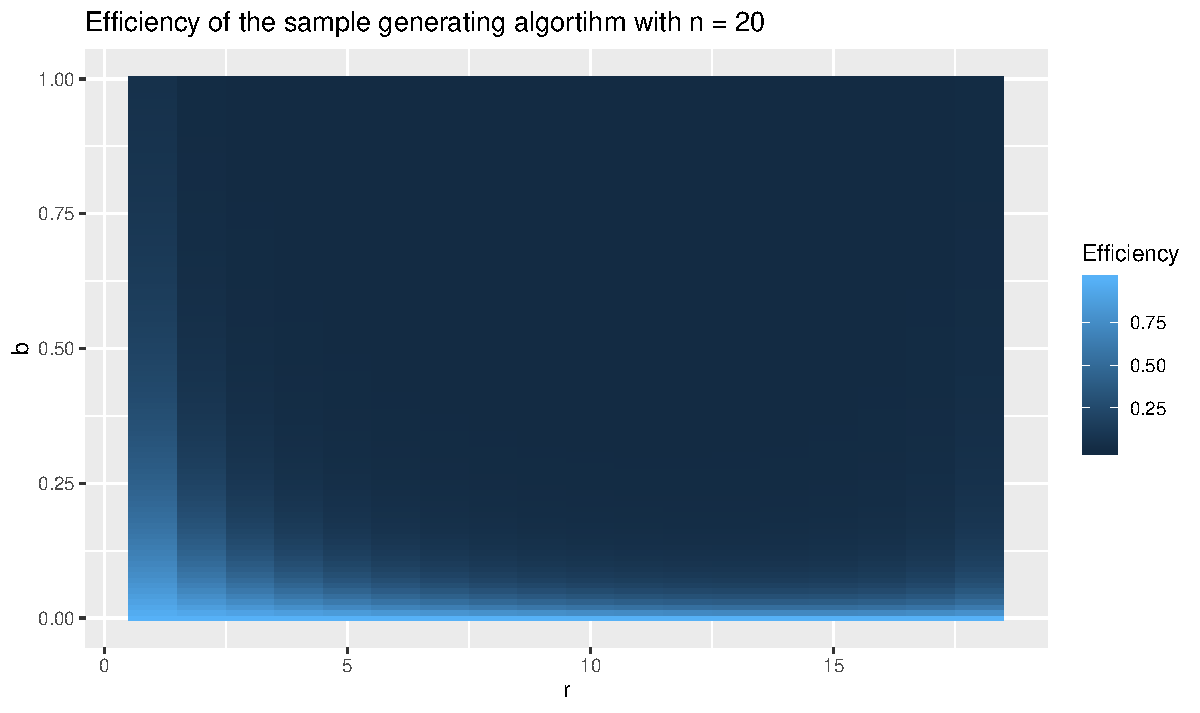
\includegraphics[scale = 0.6]{plot_eff.pdf}
    \caption{The efficiency of Algorithm\ref{algorithm: Exp Hr sample} with $n =12$}\label{Figure: efficiency}}
    {
     The efficiency of the sample generating algorithm for samples under $H_r$ with different
     contamination number $r$ and contamination rate parameter $b$. 
    }
\end{figure}

\subsection{Power Estimation} \label{sec:power est}

Let $\mathbf x_1,\ldots, \mathbf x_n$ be independent samples arose from distribution $F(\theta)$, with $\theta$ unknown. Let $\Theta$ be the parameter space
of $\theta$ and we are interested in testing $H_0 : \theta \in \Theta_0$ against $H_a: \theta \in \Theta_a = \Theta \setminus \Theta_0$. Let $C$ be a subset of the
sample space such that
\[ 
    \sup_{\theta \in \Theta_0} \P[\theta]{\mathbf X \in C} = \alpha
\]
so that hypothesis testing procedure of $H_a$ against $H_0$ of rejecting $H_0$ if $\mathbf x \in C$ would have a confidence level of $1 -\alpha$. Suppose we want to
 estimate the power of the test for a given $\theta \in \Theta_a$ which is given by $\gamma_\theta  = \P[\theta]{\mathbf x \in C}$. Consider the indicator function
 $I_\theta (\mathbf x) = \I{\mathbf x \in C}$, then $I_\theta \sim \mathrm{Ber}(\gamma_\theta)$, and so estimating $\gamma_\theta$ is equivalent to estimating the parameter of
 $I_\theta$.

 It then follows from the law of large numbers that, if $B_1,\ldots, B_N$ are random samples of $I_\theta$, then
 \[ 
     \lim_{N \to \infty} \frac{1}{N} \sumi{N} B_n \toas \E{I_\theta} = \gamma_\theta.
 \]

In particular, if $T$ is a statistic used to test the slippage alternative $H_r$ against $H_0$ with rejection region $C$ and that we are interested in
estimating the power of $T$. Let $\mathbf x_1,\ldots. \mathbf x_n$ be the random sample generated by Algorithm\ref{algorithm: Exp Hr sample}. Then,
the power of the test can be estimated by

\[ 
    \hat \gamma =  \frac{1}{n} \sumi{n} \I{T(\mathbf x_i) \in C}.
\]

It then follows from the property of the Bernoulli distribution that the standard error of $\hat \gamma_G$ is given by

\[ 
    \se(\hat \gamma) = \sqrt{\frac{\hat\gamma(1- \hat \gamma )}{n}}.
\]

\subsection{Estimation of Statistical Functions}

In this study, we are interested in estimating some unknown distribution $\overline F$ which does not have an explicit expression, but we are able to generate random sample of $\overline F$.
For this purpose, we now introduce some simulation concepts and methods that will be used latter.

\subsubsection{Empirical Distribution Functions}

With a sample of univariate data points $x_1,\ldots,x_n$ from distribution $F$, a commonly used tool to summarize the data is using histogram. 
The shape of the histogram often provides valuable information about the pdf of $F$,
for example, a bell shaped histogram may suggest normality. If we consider the cumulative histogram, then we would expect it has the shape of the CDF of $F$, and this intuition
turns out to be correct as provided in the following definition.

\begin{defn}\label{defn:ecdf}
Let $X_1,\ldots,X_n$ be a random sample of distribution $F(x)$. Then, we define the \emph{empirical distribution function}(ecdf) $\hat F_n$ to be
    \[ 
        \hat F_n(x) = \frac{1}{n} \sumi{n} \I{X_i \leqslant x}.
    \]
\end{defn}

\begin{rem}
    From this definition, we can see that $\hat F_n$ follows direct uniform distribution, as this approach has an assumption that
    each observed value is equally likely to be observed.
\end{rem}

Here, we show that ecdf $\hat F_n$ is a pointwise unbiased estimator of $F$ and give a expression for its variance.

\begin{thm}\label{thm: mean, var of ecdf}
Suppose $F$ is a cumulative distribution function and $\hat F_n$ is the empirical cumulative
distribution function based on $X_1,\ldots, X_n$. Then, for any point $ x \in \RR$,
$\hat F_n(x)$ is an unbiased estimator of $F(x)$ with variance

\begin{align*}
    \Var{\hat F_n(x)} &= \frac{F(x)(1- F(x))}{n}.
\end{align*}
\end{thm}

\begin{proof}
    Let any $x \in \RR$ be given. Then,
    \begin{align*}
        \E{\hat F_n(x)} &= \E{\frac{1}{n} \sumi{n} \I{X_i \leqslant x}}
        \\
        &=  \frac{1}{n}\sumi{n} \E{\I{X_i \leqslant x}}
        \\
        &= \P{X \leqslant x}
        \\
        &= F(x)
    \end{align*}
    and this proves that $\hat F_n(x)$ is unbiased. The variance of $\hat F_n$ is given by
    
    \begin{align*}
        \Var{\hat F_n(x)} &= \Var{\frac{1}{n} \sumi{n} \I{X_i \leqslant x}}
        \\
        &= \frac{1}{n^2} \sumi{n} \Var{\I{X_i \leqslant x}}
        \\
        &= \frac{F(x)(1- F(x))}{n}
    \end{align*}
    
    Since $\I{X_i \leqslant x} \sim \mathrm{Ber}(\P{X_i \leqslant x})$, the proof gets completed.
\end{proof}

Some characteristic $\psi$ of $F$ we are interested in, such as quantile, can often be expressed as a functional of $F$, say, $\psi = t(F)$.
It then follows from the theorem proved above and the plug-in principle that $\hat \psi = t(\hat F)$ will be an estimator of $F$, which will
be used in our study.

\subsubsection{Nonparametric Bootstrap Method} \label{sec: bootstrap}

Since $F$ is unknown, we often can not find an easy expression for the variance and bias $\hat \psi$, and so we wil use
bootstrap method to estimate it.

Recall that in this study we are focusing on Pareto and exponential distributions, and so we may assume the unknown distribution $F$ is continuous.
Then, it follows from the fact that $F(X) \sim \mathcal U(0,1)$ for any continuous random variable $X$ with cdf $F$; so, we can
use the inverse transformation method to simulate $\hat F$. More specifically, we can simulate iid samples $U_1,\ldots, U_n$ from $\mathcal U(0,1)$
distribution, then the corresponding $X_1,\ldots, X_n$ of $\hat F_n$ is generated as
\[ 
    X_i = x_{(i)} \quad \text{if} \quad \frac{i-1}{n} < U_i \leqslant \frac{i}{n}, \quad i = 1,\ldots,n,
\]

where $x_{(i)}$ is taken to be the $i^{\text{th}}$ ordered value of the support of $\hat F_n$. It follows from the definition of $\hat F_n$ given
in Definition \ref{defn:ecdf} that simulating sample from $\hat F_n$ is equivalent to taking a random sample from the support of $\hat F$ with replacement.
Hence, we can generate random samples of $\hat F_n$ by sampling from the support of $\hat F_n$, and we denote this by
$\mathbf X^*_1,\ldots, \mathbf X^*_B$. We can obtain the bootstrap estimates $\hat \psi_b = t(\mathbf X^*_b)$, for $b =1,\ldots, B$.
Then, we can estimate the bias and variance of $\hat \psi$ by

\begin{align}
    \hat b(\hat \psi) &= \frac{1}{B} \sum_{b=1}^B (\hat \psi_b - \hat \psi), \label{eqn: boot bias}
    \\
    \widehat{\mathrm{Var}}[\hat{\psi}] &= \frac{1}{B-1} \sum_{b=1}^B \left(\hat \psi - \overline{\hat \psi_b}\right)^2. \label{eqn: boot var}
\end{align}


\chapter{Exact Distributions of Discordancy Test Statistics under $H_r$ } \label{chapt: Discordancy Tests}

In this chapter we derive the exact distributions of the test statistics given by Zerbet and Nikulin \cite{zerbet2003new} and  Jabbari Nooghabi \cite{jabbari2019detecting}
under the slippage alternative $H_r$.

\section{Discordancy Tests for Exponential Samples}

Recalling the contamination model and slippage hypothesis introduced in the Definition \ref{defn: slippage Hr}, here
we consider the case where the underline distribution is $\mathrm{Exp}(\theta)$ with distribution function $F(x;\theta) = \P{X \leqslant x} = 1 -\exp{-x/\theta}$,
and the contaminated model is $\overline F = \mathrm{Exp}(\theta/b)$ for some unknown constant $b$, where $0 < b \leqslant 1$.

Zerbet and Nikulin \cite{zerbet2003new} proposed the following statistic to test $H_r$ against $H_0$:

\begin{align} \label{eqn: Z_r}
    Z_r = \frac{X_{(n-r)} - X_{(1)}}{\sum_{j=n-r+1}^n (X_{(j)}) - X_{(1)})}.
\end{align}

Since we are assuming $b <1$, under $H_r$, the test statistic $Z_r$ given in \eqref{eqn: Z_r} has the property that

\begin{align*}  
    \lim_{b \to \infty} \E{Z_r} &= \lim_{b \to \infty} \E{\frac{X_{(n-r)} - X_{(1)}}{\sum_{j=n-r+1}^n (X_{(j)}) - X_{(1)})}}
    \\
    &\leqslant \lim_{b \to \infty} \E{\frac{X_{(n-r)}}{X_{(n)} - X_{(1)}}}
    \\
    &= 0,
\end{align*}
for $X_{(n-r)}$ and $X_{(1)}$ are arising from $\mathrm{Exp}(\theta)$ and $X_{(n)}$ is arising from $\mathrm{Exp}(\theta/b)$ under $H_r$. 
Therefore, one should reject $H_0$ if $Z_r < z_c$, where $z_c(\alpha)$ is the $\alpha$ quantile of $Z_r$. So, we have corrected the direction of the test claim in \cite{zerbet2003new}, where they claimed the test direction is a upper tail test.
Here, we derive its distribution, which is the corrected version of Theorem 1 proved in \cite{zerbet2003new}.

\subsection{Distribution of $Z_r$}

\begin{thm} \label{thm: distribution of Z_r}

The distribution of the statistic $Zr$, under $H_r$, is given by
    \begin{align*}
        \P{Z_r < Z \mid H_r} &\begin{aligned}[t]
            &= \frac{b^{r}\Gamma(rb+n+r)}{\Gamma(rb+1)} 
            \\
            &\times \sum_{j=2}^{n-r} \frac{(-1)^{n-j-r}\{b^{-r} - [(rb + n-r-j+1)(z/(1-rz))+b]^{-r}\}}{(j-2)!(n-j-r)!(rb+n-r-j+1)}, \qquad 0 < x < \frac{1}{r}.
        \end{aligned}
    \end{align*}
\end{thm}

\begin{proof}
    Suppose $H_r$ holds and consider the random variable $U_r$ given by
    \[ 
        U_r = \frac{X_{(n-r)} - X_{(1)}}{\sum_{j=n-r+1}^n (X_{(j)}) - X_{(n-r)})}.
    \]
    Then
    \begin{align} \label{eqn: relation between Zr and Ur}
        \frac{1}{Z_r} - \frac{1}{U_r} &= \frac{1}{X_{(n-r)} - X_{(1)}}\sumj{r} X_{(n-r)} - X_{(1)} = r ,
    \end{align}
    so that $U_r = \frac{Z_r}{1-r}$. We obtain the distribution of $Z_r$ by considering the distribution of $U_r$. Let

    \[ 
        V = X_{(n-r)} - X_{(1)} \qquad \text{and} \qquad W = \sum_{j=n-r+1}^n X_{(j)} - X_{(n-r)}.
    \]
    Then the test statistic $Z_r = V/W$. Let $Y_j = X_{(j)} - X_{(1)}$. Because
    \begin{align*}
        \sumj[2]{n-r} Y_j &= \sumj[2]{n-r} X_{(j)} - X_{(j-1)}
        \\
        &= \sumj[2]{n-r} X_{(j)} - \sumj[2]{n-r} X_{(j-1)}
        \\
        &= X_{(n-r)} - X_{(1)} + \sumj[1]{n-r-1} X_{(j)} - \sumj[1]{n-r-1} X_{(j)}
        \\
        &= X_{(n-r)} - X_{(1)}
    \end{align*}
    and
    \begin{align*}
        \sum_{j = n-r+1}^n (n-j+1)Y_j &= \sum_{j = n-r+1}^n  X_{(j)} - X_{(j-1)}
        \\
        &= \sum_{j = n-r+1}^n  X_{(j)} - \sum_{j = n-r}^{n-1}  X_{(j-1)}
        \\
        &= \sum_{j = n-r+1}^n  X_{(j)} - \sum_{j = n-r}^{n-1}  X_{(j-1)}
        \\
        &= (n-n+1)X_{(n)} -(n-n+r-1+1) X_{(n-r+1)} + \sum_{j = n-r}^{n-1}  (n-j+1)X_{(j)} - (n-j)X_{j}
        \\
        &= X_{(n)} - rX_{(n-r)} + \sum_{j=n-r}^{n-1} X_{(j)}
        \\
        &= \sum_{j=n-r}^n X_{(j)} - X_{(n-r)},
    \end{align*}
    we have
   \begin{align} \label{eqn : Z_r in terms of Y}
    Z_r = \frac{V}{W} = \frac{\sum_{j=2}^{n-r} Y_j}{\sum_{j=n-r+1}^n (n-j+1)Y_j}.
   \end{align}
    The joint characteristic function $(V,W)$ is

    \begin{align*}
        \varphi_{V,W}(t,z) &= \E{ \exp{i(Vt + Wz)}} \\
        &= \E{ \exp{i\left( \sumj[2]{n-r} Y_j t + \sum_{j=n-r+1}^n (n-j+1)Y_jz\right)}}
        \\
        &=\begin{aligned}[t]
            &\int_{\RR^{n-1}} \exp{i\left( \sumj[2]{n-r} Y_j t + \sum_{j=n-r+1}^n (n-j+1)Y_jz\right)}
            \\
            &\times f_{(Y_2,\ldots,Y_n)}(y_2,\ldots,y_n) \dd{y_2}\cdots\dd{y_n}.
        \end{aligned} \\
   \end{align*}

   It follows from Lemma \ref{Lemma: order statistic transformation} that $Y_j, j = 1, \cdots, n - r$, follows $\mathrm{Exp}(\theta(rb+n-r-j+1))$
   and $Y_{n-r+j}$ follows $\mathrm{Exp}((\theta/b)(r-j+1)^{-1})$ distribution. Let $a_j = \theta(rb+n-r-j+1)^{-1}$ and $b_j =(\theta/b)(r-j+1)^{-1}$.
   We can then write $\varphi_{(V,W)}(t,z)$ as
   \begin{align*}
    \varphi_{V,W}(t,z) &= \begin{aligned}[t]
        &\int_{\RR^{n-1}} \exp{it( \sumj[2]{n-r} Y_j)}\left[\prodk[2]{n-r} \frac{1}{a_k}e^{-yk/ak}\right]
        \\
        &\times \exp{iz \sumj[n-r+1]{n}(n-j+1)y_j} \left[ \prodk{r} \frac{1}{b_k}e^{-y_{n-r+1}/b_k}\right] \dd{y_2}\cdots \dd{y_n}
    \end{aligned}
    \\
      &= \begin{aligned}[t]
        & \prodj[2]{n-r} \int_0^\infty  \frac{1}{a_j}\exp{- \frac{y_j}{a_j} + ity_j} \dd{y_j}
        \\
        &\times \prodj{r} \int_0^\infty \frac{1}{b_j} \exp{-iz(r-j+1)y_{n-r+j} -y_{n-r+j}/b_j} \dd{y_{n-r+j}}
    \end{aligned}
    \\
    &= \begin{aligned}[t]
        & \prodj[2]{n-r} \int_0^\infty  \frac{1}{a_j}\exp{- \frac{y_j}{a_j} + ity_j} \dd{y_j}
        \\
        &\times \prodj{r} \int_0^\infty \frac{1}{b_j} \exp{-y_{n-r+j}\left(\frac{1}{b_j}-iz(r-j+1)\right)} \dd{y_{n-r+j}}
    \end{aligned}
    \\
    &= \left[\prodj[2]{n-r} \frac{1}{a_j}(1/a_j -it)^{-1}\right] \times \left[\prodj{r}\frac{1}{b_j}(1/b_j -iz(r-j+1))^{-1}\right].
   \end{align*}
   
   It then follows from Lemma \ref{Lemma : inversion formula} that the joint pdf of $(V,W)$ is given by 

   \begin{align} \label{eqn: joint pdf f(vw)}
       f_{(V,W)}(v,w) &= \frac{1}{(2\pi)^2} \int_0^\infty \int_0^\infty \varphi_{(V,W)}(t,z) \exp{it(tv+wz)} \dd{t}\dd{z} \nonumber
       \\
       &= \frac{1}{(2\pi)^2} \int_0^\infty \left[ \prodj[2]{n-r} \frac{1}{a_j}(1/a_j -it)^{-1}\exp{itv}\dd{t}\right] \times \int_0^\infty \left[\prodj[1]{r}\frac{1}{b_j}(1/b_j -iz(r-j+1))^{-1}e^{-iwz}\dd{z}\right]
   \end{align}

   To simplify \eqref{eqn: joint pdf f(vw)}, we first use Lemma \ref{Lemma: partial fraction}
   to obtain

   \begin{align*}
      \prodj[2]{n-r} \frac{1}{1/a_j -it} &= (-1)^{n-r-1} \prodj[2]{n-r} \frac{1}{it-1/a_j}
      \\
      &= (-1)^{n-r-1} \sumj[2]{n-r} \frac{1}{it -1/a_j} \prod_{{i\neq 1, i\neq j}}^{n-r} \frac{1}{1/a_j - 1/a_i}
      \\
      &= (-1)^{n-r-1} \sumj[2]{n-r} \frac{1}{it -1/a_j} \prod_{{i\neq 1 , i\neq j}}^{n-r} \frac{1}{\theta^{-1}(i-j)}
      \\
      &= (-1)^{n-r-1} \sumj[2]{n-r} \frac{\theta^{n-r-2}}{it -1/a_j} \left[\prodi[2]{j-1}\frac{1}{1-j}\right] \left[\prodi[j+1]{n-r}\frac{1}{1-j}\right]
      \\
      &= (-1)^{n-r-1} \sumj[2]{n-r} \frac{\theta^{n-r-2}}{it -1/a_j} \left[\frac{(-1)^{j+2}}{((j-2)!)}\right] \left[\frac{1}{(n-r-j)!}\right]
      \\
      &= \sum_{j=2}^{n-r} \frac{(-1)^{n+j-r-1}\theta^{n-r-2}}{(it-1/a_j)(j-2)!(n-j-r)!},
   \end{align*}

    
   \begin{align*}
       \prodj{r} (1/b_j -iz(r-j+1))^{-1} &= \prodj{r}\left(\frac{b}{\theta}(r-j-1)-iz(r-j+1)\right)^{-1}
       \\
       &= \prodj[1]{r}((b/\theta -iz)(r-j+1))^{-1}
       \\
       &= (b/\theta -iz)^{r} \prodj[1]{r} (r-j+1)^{-1}
       \\
       &= \frac{(b/\theta -iz)^{r}}{r!},
   \end{align*}

   \begin{align*}
       \prodj{r} \frac{1}{a_j} &= \prodj[2]{n-r} \frac{rb+n -r -j +1}{\theta}
       \\
       &= \frac{1}{\theta^{n-r-1}} \frac{\Gamma(rb+n-r)}{\Gamma(rb+1)},
   \end{align*}
   and
   \begin{align} \label{eqn: prod 1/b_j}
    \prodj{r} \frac{1}{b_j} = \prodj{r} \frac{b}{\theta}(r-j+1) = \left(\frac{b}{\theta}\right)^r r!.
   \end{align}
    
   We can then express the $f_{V,W}(v,w)$ given in \eqref{eqn: joint pdf f(vw)} as
   \[ 
       f_{(V,W)}(v,w) = \left[ \frac{1}{(2\pi)^2} \sumj[2]{n-r} \frac{\Gamma(rb+n-r)(-1)^{n+j-r-1}}{\Gamma(rb+1)(j-2)!(n-j-r)!}\int_0^\infty \frac{e^{-iv}}{it-1/a_j}\dd{t}\right] \times \left[ \left(\frac{b}{\theta}\right)^{r+1} \int_0^\infty \frac{e^{-iwz}}{(b/\theta -iz)^r}\dd{z}\right].
   \]

   We now claim that
   \[ 
    \int_0^\infty \frac{e^{-iwz}}{(b/\theta - iz)^r} \dd{z} = \frac{2\pi w^{r-1}}{(r-1)!} e^{-wb/\theta}.
    \]
   To show that the above integration identity holds, let $X$ be a random variable having $\mathrm{Gamma}(r,\theta/b)$ distribution, with the pdf $p(x)$ and characteristic function $f(x)$ as
   \[ 
       p(x) =  \frac{w^{r-1}e^{-w/b}}{\Gamma(r)\theta^{\alpha} },\quad x>0, \qquad \text{and} \qquad f(x) = (1-ix \theta/b)^{-r}.
   \]
   Then, it follows from Lemma \ref{Lemma : inversion formula} that
   \begin{align*}
       && 2\pi p(w) &=  \int_{-\infty}^{\infty} e^{-izw} f(t) \dd{z}
       & \\
      \iff && 2\pi \frac{w^{r-1}e^{-w\theta/b}}{(\theta/b)^r(r-1)!} &=\int_0^\infty \frac{e^{-iwz}}{(1-iz\theta/b)^r} \dd{z}
      & \\
      \iff && 2\pi \frac{w^{r-1}e^{-w\theta/b}}{(r-1)!} &= \int_0^\infty \frac{e^{-iwz}}{(b/\theta)^r  (1-iz\theta/b)^r} \dd{z}
      & \\
     \iff &&  2\pi \frac{w^{r-1}e^{-w\theta/b}}{(r-1)!} &= \int_0^\infty \frac{e^{-iwz}}{(b/\theta - iz)^r} \dd{z}   
   \end{align*}
   which proves the claim.

   Because $Z_r = V/W$, therefore we can obtain the distribution of $Z_r$ by direct integrate $f_{V,W}(v,w)$ as follows:

   \begin{align*}
    \P{U_r < u} &= \P{ \frac{V}{W} <u}
    \\
    &= \P{V < uW}
    \\
    &= \int_0^\infty \int_0^{uw} f_{(V,W)}(v,w) \dd{v} \dd{w}.
\end{align*}

It follows from the Lemma \ref{Lemma : inversion formula} and the characteristic function of $\mathrm{Exp}(1/a_j)$ that
\[ 
    \int_0^\infty \frac{e^{-itv}}{it- 1/a_j} \dd{t} = -a_j \int_0^\infty \frac{e^{-itv}}{1-it a_j} \dd{t} = -2\pi \exp{-\frac{1}{a_j} v},
    \]
    
    and also by Lemma \ref{Lemma : inversion formula}, we can simplify $f_{V,W}(v,w)$ to

\begin{align*}
    f_{V,W}(v,w) &= \begin{aligned}[t]
        &\frac{\Gamma(rb+n-r)}{\Gamma(rb+1)} \left(\frac{b}{\theta}\right)^{r+1} \frac{1}{(r-1)!}
        \\
        &\times \sumj[2]{n-r} \frac{(-1)^{n+j-r}}{(j-2)!(n-j-r)!} g(v,w),
    \end{aligned}
\end{align*}
where
\[ 
    g(v,w) = w^{r-1}\exp{-\frac{v}{a_j} - \frac{b}{\theta} w}.
\]

Since
\begin{align*}
    \int_0^\infty \int_0^{uw} g(v,w) \dd{v}\dd{w} &= \int_0^\infty w^{r-1} \exp{-\frac{b}{\theta}w}(-a_j)\left[\exp{-\frac{u}{a_j}w}-1\right] \dd{w}
    \\
    &= \begin{aligned}[t]
    & -a_j \Bigg[ \int_0^\infty w^{r-1} \exp{- \left( \frac{b}{\theta} + \frac{1}{a_j}u\right)w} \dd{w}
        \\
    &- \int_0^\infty w^{r-1} \exp{- \frac{b}{\theta}w} \dd{w} \Bigg]
    \end{aligned} 
    \\
    &= -a_j \left[\Gamma(r)\left(\frac{b}{\theta} + \frac{u}{a_j}\right)^{-r} - \Gamma(r)\left( \frac{b}{\theta}\right)^{-r} \right]
    \\
    &= -a_j (r-1)! \left[\left(\frac{b + u\theta/a_j}{\theta}\right)^{-r} - \left(\frac{b}{\theta}\right)^{-r}\right]
    \\
    &= a_j (r-1)!\theta^r \left[b^{-r} - [u\theta/a_j + b]^{-r} \right],
\end{align*}

we have
\begin{align*}
    \int_0^\infty \int_0^{uw} f_{(V,W)}(v,w) \dd{v}\dd{w} &=\frac{\Gamma(rb+n-r)}{\Gamma(rb+1)} \left(\frac{b}{\theta}\right)^{r+1} \frac{1}{(r-1)!} \times \sumj[2]{n-r} \frac{(-1)^{n+j-r}}{(j-2)!(n-j-r)!} \int_0^\infty \int_0^{uw} g(v,w) \dd{v}\dd{w}
    \\
     &= \begin{aligned}[t]
        &\frac{\Gamma(rb+n-r)}{\Gamma(rb+1)} \left(\frac{b}{\theta}\right)^{r+1} \frac{1}{(r-1)!} \sumj[2]{n-r} \frac{(-1)^{n-j-r}}{(j-2)!(n-j-r)!}\\
    & \times a_j (r-1)!\theta^r \left[b^{-r} - [u\theta/a_j + b]^{-r} \right]
     \end{aligned}
    \\
    &= \frac{\Gamma(rb+n-r)}{\Gamma(rb+1)} \frac{b^{r+1}}{\theta} \sumj[2]{n-r} \frac{(-1)^{n-j-r}}{(j-2)!(n-j-r)!} a_j \left\{b^{-r} - [u\theta/a_j + b]^{-r} \right\}
    \\
    &=\frac{b^{r+1}\Gamma(rb+n-r)}{\Gamma(rb+1)}  \sumj[2]{n-r} \frac{(-1)^{n-j-r}}{(j-2)!(n-j-r)!} \frac{\left[b^{-r} -(u\theta/a_j + b)^{-r} \right]}{\theta/a_j}.
\end{align*}
Then, using the fact that $\theta/a_j = (rb+n-r-j+1)$, the above equality becomes
\[ 
    \P{U_r < u} = \int_0^\infty \int_0^{uw} f_{(V,W)}(v,w) \dd{v}\dd{w} =  \frac{b^{}\Gamma(rb+n-r)}{\Gamma(rb+1)} \sumj[2]{n-r} \frac{(-1)^{n-j-r}\{b^{-r}  - [(rb+n-r-j+1)u + b]^{-1}\}}{(j-2)!(n-j-r)!(rb+n-r-j+1)},
\]
and then the required result follows from $U_r = \frac{Z_r}{1-r}$.
\end{proof}

\begin{rem}
    We remark that the mistake in \cite{zerbet2003new} has been corrected by Mehdi Jabbari Nooghabi,
    since he proved an analogous result for Pareto distribution in \cite{jabbari2019detecting}, where $b$  corresponds to $\beta$ and $r$
    corresponds to $k$.
\end{rem}  


\section{Discordancy Tests for Pareto Samples}

In the previous section, we investigated a statistic test proposed by
Zerbet and Nikulin to test the slippage alternative hypothesis for exponential samples. It turns out
that the same kind of statistics can be easily adapted to test the slippage alternative for Pareto distribution.
This was introduced by Jabbari Nooghabi \cite{jabbari2019detecting}.

To be consistent with the notation used in \cite{jabbari2019detecting}, we will consider the slippage alternative introduced
in the Definition \ref{defn: slippage Hr} with $F = \mathrm{Pareto}(\alpha, \theta)$ and $\overline F = \mathrm{Pareto}(\alpha \beta, \theta)$ with $\beta <1$.

\subsection{Test Statistics}

Jabbari Nooghabi \cite{jabbari2019detecting} proposed the statistic $\tilde Z_k$ and $\tilde R_r$ to test $H_r$ against $H_0$ for Pareto samples, where

\[ 
    \tilde Z_r = \frac{\ln(X_{(n-r)}) - \ln(X_{(1)})}{\sum_{j = n - r + 1}^n (\ln(X_{(j)}) - \ln(X_{(1)}))}
\]
    
    and
\[
       \tilde R_r = \frac{\ln(X_{(n-r)}) - \ln(X_{(1)})}{\ln(X_{(n)}) - \ln(X_{(n-r+1)})}.
\]
        
In \cite{jabbari2019detecting}, the test statistic $\tilde R_r$ was first introduced, and was actually used as $1 - \tilde R_r$.  Since $1 - R_r$ does not
have any theoretical advantage over $\tilde R_r$, but $\tilde R_r$ has a non-negative support and better interpretability, we will use $R_r$ as
the test statistic here.


% Since we have derived the exact distribution of $Z_r$ in Theorem \ref{thm: distribution of Z_r}, therefore we the
% power function for $Z_r$ can be calculate by

% \[ 
%     \gamma_{Z_r}(b) = \P{Z_r < z_\alpha \mid H_r} = 1 - F_{Z_r}(z_\alpha; b),
% \]
% where $z_\alpha$ is the corresponding critical values found in the Table \ref{table: Zr critical values}.



\begin{thm}
    Let $X_1,\ldots, X_n$ be a collection of independent Pareto random variable, and
    under slippage alternative hypothesis $H_r$. Then the distribution of statistic $\tilde Z_r$ is given by
    \begin{align*}
        \P{\tilde Z_r < z \mid H_r} \begin{aligned}[t]
            &= \frac{\beta^{r}\Gamma(r\beta+n-r)}{\Gamma(rb+1)} \sum_{j=2}^{n-r} \sum_{i=2}^r  \frac{(-1)^{n+i+j-2}}{(n-r-j)!(j-2)!(r-i)!(i-2)!}
            \\
            & \times \frac{[ \beta(r -i+1)]^{-1} - [\beta(x-i+1) + z(r\beta + n -r -j +1)]^{-1}}{r\beta + n -r - j+ 1}.
        \end{aligned}
    \end{align*}
\end{thm}

\begin{proof}
    We first note that, for any $1 < j , l <n$, we have
    \[ 
        \ln(X_{(j)}/\theta) - \ln(X_{(l)}/\theta) = \ln(X_{(j)}) - \ln(X_{(l)})
    \]
        and so  the result follows from the form of $Z_r$ and $\tilde Z_r$ and the
        use of Theorem \ref{thm: distribution of Z_r} and Corollary \ref{cor: distribution of log Pareto OS under Hr}.
\end{proof}
    
    
\subsection{Distribution of $\tilde R_r$ }
    In this section, we will derive the distribution of $\tilde R_r$ under $H_r$ as given in the following theorem.

    \begin{thm} \label{thm: distribution of  R_r}
        The distribution of the statistic $\tilde R_r$ under $H_r$ is given by
    \begin{align*}
        \P{\tilde R_r< x \mid H_r} &\begin{aligned}[t]
            &= \frac{\beta^{r}\Gamma(r\beta+n-r)}{\Gamma(rb+1)} 
            \\
            &\times \sum_{j=2}^{n-r} \frac{(-1)^{n-j-r}\{\beta^{-r} - [(r\beta + n-r-j+1)(x/(1-rx))+\beta]^{-r}\}}{(j-2)!(n-j-r)!(r\beta+n-r-j+1)} \qquad 0 < x < \frac{1}{r}.
        \end{aligned}
    \end{align*}
    \end{thm}



    
\begin{proof}
    We will prove the result using characteristic function. Let $X_{(1)},\ldots,X_{(n)}$ be the order statistics from the sample under $\overline{H}_r$. Then, $\tilde R_r$ can be written as
    \[ 
        \tilde R_r = \frac{\sum_{j=2}^{n-k} Y_j}{\sum_{j=n-k+2}^n Y_j} = \frac{P}{Q}
    \]
    where $Y_j = \ln(X_{(j)}) - \ln(X_{(j-1)})$, for $j > 1$. It then follows from Lemma \ref{Lemma: order statistic transformation} and Lemma \ref{lem: log of Pareto is exp}
    that the joint distribution of $P$ and $Q$ is given by
    \begin{align*}
        \phi_{P,Q}(t,s) &= \prod_{j=2}^{n-r} \phi_{Y_j} \prod_{j=2}^{r} \phi_{Y_j}
        \\
        &= \prod_{j=2}^{n-r} \left[\frac{1}{a_j}\left(\frac{1}{a_j}-it\right)\right] \prod_{j=2}^{r} \left[\frac{1}{b_j}\left(\frac{1}{b_j}-is\right)\right],
    \end{align*}
    where $a_j = [\alpha(r\beta + n - r -j+1)]^{-1}$ and $b_j = [\alpha \beta(r-j+1)]^{-1}$. Using Lemma \ref{Lemma : inversion formula}, we have the joint density function of $U$ and $V$ as
    \[ 
        f_{P,Q}(p,q)= \frac{1}{(2\pi)^2} \int_0^\infty \left[ \prodj[2]{n-r} \frac{1}{a_j}(1/a_j -it)^{-1}\exp{-itp}\dd{t}\right] \times \int_0^\infty \left[ \prodj[2]{n-r} \frac{1}{b_j}(1/b_j -it)^{-1}\exp{-isq}\dd{t}\right].
    \]
    To simplify $f_{P,Q}$, we first use Lemma \ref{Lemma: partial fraction} to calculate

    \begin{align*}
        \prod_{j=2}^k \frac{1}{1/b_j - is} &= (-1)^{r} \prodj[2]{r} \frac{1}{it-1/b_j}
        \\
        &= (-1)^{r-1} \sum_{j=2}^r \frac{1}{is - 1/b_j} \prod_{i=2}^k \frac{1}{\alpha \beta(k-i)}
        \\
        &= (-1)^{r-1} \frac{1}{(\alpha\beta)^{r-2}} \sum_{j=2}^k \frac{1}{is - 1/b_j} \prod_{k=2}^r \frac{1}{k-i}
        \\
        &= (-1)^{r-1} \frac{1}{(\alpha\beta)^{r-2}} \sum_{j=2}^k \frac{1}{is - 1/b_j} \frac{(-1)^{j-2}}{(j-2)!(k-j)!}
        \\
        &= \sum_{j=2}^r \frac{(-1)^{r+j-1}}{(is-1/b_j)(j-2)(r-j)!(\alpha \beta)^{r-2}}.
    \end{align*}
    It also follows from \eqref{eqn: prod 1/b_j} that
    \[ 
        \prod_{j=2}^r \frac{1}{b_j} = (r-1)!(\alpha\beta)^{r-1}.
    \]
    Therefore, with the product identity derived in the proof of Theorem \ref{thm: distribution of Z_r} we
    obtained the simplified pdf for $f(p,q)$ is given by

    \begin{align*}
        f_{P,Q}(p,q) &= \frac{\alpha \Gamma(r \beta + n -r)}{\Gamma (r \beta +1)} \sum_{j=2}^{n-r} \frac{(-1)^{n-r+j-1}}{(j-2)(n-r-j)!} \exp{-n_jp} \times \alpha \beta(r-1)! \sum_{i=1}^r \frac{(-1)^{n-r+j-1}}{(r-1)!(i-2)!}\exp{-m_iq},
    \end{align*}
    where $n_j = -\alpha(r \beta + n -r - j+ 1)$ and $m_i = -\alpha \beta(r-i+1)$. Then, the distribution
    for $\tilde R_r$ is given by
    \begin{align*}
        \P{\tilde R_r< x} &= \frac{\alpha ^2\beta \Gamma(r \beta + n -r )}{\Gamma(r \beta +1)} \sum_{j=2}^{n-k} \sum_{i=2}^r \frac{-1^{n+j+i-2}}{(n-r-j)!(j-2)!(r-1)!(i-2)!} \int_0^\infty \int_0^{rq} \exp{-\alpha n_j p + -\alpha m_i q} \dd{p} \dd{q}
        \\
        &= \frac{\alpha^2 \beta \Gamma(r \beta + n -r )}{\Gamma(r \beta +1)} \sum_{j=2}^{n-k} \sum_{i=2}^r \frac{-1^{n+j+i-2}}{(n-r-j)!(j-2)!(r-1)!(i-2)!} \alpha^{-2} \frac{x}{m_i(n_jx +m_i)}
        \\
        &= \frac{\beta^{r}\Gamma(r\beta+n-r)}{\Gamma(rb+1)} \sum_{j=2}^{n-r} \sum_{i=2}^r  \frac{(-1)^{n+i+j-2}}{(n-r-j)!(j-2)!(r-i)!(i-2)!} \times \frac{m_i^{-1} - ( m_i + x n_j)^{-1}}{n_i}
        \\
        & \begin{aligned}[t]
            &= \frac{\beta^{r}\Gamma(r\beta+n-r)}{\Gamma(rb+1)} \sum_{j=2}^{n-r} \sum_{i=2}^r  \frac{(-1)^{n+i+j-2}}{(n-r-j)!(j-2)!(r-i)!(i-2)!}
            \\
            & \times \frac{[ \beta(r -i+1)]^{-1} - [\beta(x-i+1) + x(r\beta + n -r -j +1)]^{-1}}{r\beta + n -r - j+ 1}.
        \end{aligned}
    \end{align*}

\end{proof}


\chapter{Simulation Study} \label{chapt: Simulation Study}

In this chapter, we will use simulation method introduced earlier in Chapter \ref{chapt: Simulation Study} to numerically verify the exact distributions of the following discordancy test statistics
that can be used to test the slippage alternative $H_r$ when we are given random sample $\mathbf X = (X_1,\ldots, X_n)$, where each $X_i$ is known to be
independent exponential with location parameter. For this simulation study, we have focused on the following three test statistics:

\begin{align*}
    D_r(\mathbf X) &= \frac{X_{(n)} - X_{(n-r)}}{X_{(n)}},  \\
    R_r(\mathbf X) &= \frac{X_{(n-r)} - X_{(1)}}{X_{(n)} - X_{(n-r+1)}}, \\
    Z_r(\mathbf X) &= \frac{X_{(n-r)} -X_{(1)}}{\sum_{j = n - r + 1}^n X_{(j)} - X_{(1)}},
\end{align*}
where $Z_r$ is first introduced by Zerbet and Nikulin in \cite{zerbet2003new}. Its correct distribution under $H_r$ has been given in Theorem \ref{thm: distribution of Z_r}.
The statistic $R_r$ was introduced by Jabbari Nooghabi in \cite{jabbari2019detecting} as $J\!Z_r = 1- \tilde R_r$, where $J\!Z_r$ is the statistic they proposed and
$\tilde R_r$ is given by

\begin{align*}
    \tilde R_r(\mathbf Y)  &= \frac{\ln(Y_{(n-r)}) - \ln(X_{(1)})}{\ln(Y_{(n)}) - \ln(Y_{(n-r+1)})}.
\end{align*}
The corrected distribution of $\tilde R_r$ under $H_r$ has been presented in Theorem \ref{thm: distribution of R_r}. The statistic $D_r$ is the classical Dixon statistic, which
we use as a reference for power comparison.

Motivated by Corollary \ref{cor: distribution of order stats}, we also consider the following test statistics: 

\begin{align*}
   \tilde D_r(\mathbf Y) &= \frac{\ln(Y_{(n)}) - \ln(Y_{(n-r)})}{\ln(Y_{(n)})}, \label{eqn: modified Dr} \\
    \tilde Z_r(\mathbf Y) &= \frac{\ln(Y_{(n-r)}) -\ln(Y_{(1)})}{\sum_{j = n - r + 1}^n \ln(Y_{(j)}) - \ln(Y_{(1)})}
\end{align*}

Then, it follows from Corollary \ref{cor: distribution of log Pareto OS under Hr} that $\tilde D_r$, $\tilde R_r$ and $\tilde Z_r$ will have the same distribution
as $D_r$, $R_r$ and $Z_r$ if $\mathbf Y = (Y_1,\ldots, Y_n)$, where each $Y_i$ is Pareto random variable with scale parameter $\theta$
and shape parameter the same as the scale parameter of $X_i$. Therefore, $\tilde D_r$, $\tilde R_r$ and $\tilde Z_r$ can be used to
test $H_r$ for Pareto random samples, and they will have the same critical values and power as $D_r$, $R_r$ and $Z_r$ respectively.

To avoid confusion, in this chapter, we assume the number of contanminants is $r$, observation sample size is $n$
for both exponential and Pareto case. When consdering slippage alternative, $F$ and $\overline{F}$ in Definition \ref{defn: slippage Hr} are taken to be $\mathrm{Exp}(\theta)$
and $\mathrm{Exp}(\theta/b)$, respectively, for exponential case; $F$ and $\overline{F}$ are taken to be $\mathrm{Pareto}(\alpha, \theta)$
and $\mathrm{Pareto}(\alpha b, \theta)$, respectively, for Pareto case. The parameter $b$ is assumed to be a unknown real number in $(0,1)$;  $\alpha$ and $\theta$ are both fixed but unknown. 
As done in \cite{zerbet2003new}, we taken sample size $n$ to ve $12$ and number of contanminants as $r$ to be $3$ for the illustrative power comparison.





\section{Numerical Verification of the Exact Distributions}

In Chapter \ref{chapt: Discordancy Tests}, we have derived the exact distribution of $\tilde R_r$ in Theorem \ref{thm: distribution of R_r} and the exact distribution of $Z_r$ in
Theorem \ref{thm: distribution of Z_r}, we will numerically verify them through simulation studies, where
simulation sample size is $B = 5000$. The sample generated are depicted in Figure \ref{Figure: cdf of Zr}.
As can be seen from the figure, the theoretical distribution agrees with the empirical distribution. 

It follows from Theorem \ref{thm: mean, var of ecdf} that the standard error of empirical distribution $\hat F(x)$ is estimated by 

\[   
\se(\hat F(x)) = \sqrt{\frac{1}{B}\hat F(x) (1- \hat F(x))},
\]
and the $95\%$ confidence intervals are obtained by assuming that the distribution
of $F(x) -\hat F(x)$ follows normal, and so we have the $95\%$ normal CI for $F(x)$ to be

\[ 
    \hat F(x) \pm \sqrt{\frac{1}{B}\hat F(x) (1- \hat F(x))}.
\]

Similarly, we generated Pareto samples and compare the theoretical cdf and ecdf and verify the
theoretical distribution of $\tilde R_r$ given in Theorem \ref{thm: distribution of R_r} in Figure \ref{Figure: cdf of Rk}. Since Pareto distribution
have a very long tail, we have taken the log of the order statistics in Panel A for illustrataion purpose. One may notice that Panel A of
Figure \ref{Figure: cdf of Rk} and Figure \ref{Figure: cdf of Zr} are exact the same, and this is not a coincidence. It follows from
the Corollary \ref{cor: distribution of log Pareto OS under Hr} that the logarithm distribution of the order statistic is the same
as that of exponential distribution with appropriate parameter, and we have used the same seed for all the simulation study.

\begin{figure}[hbtp]
    \centering
    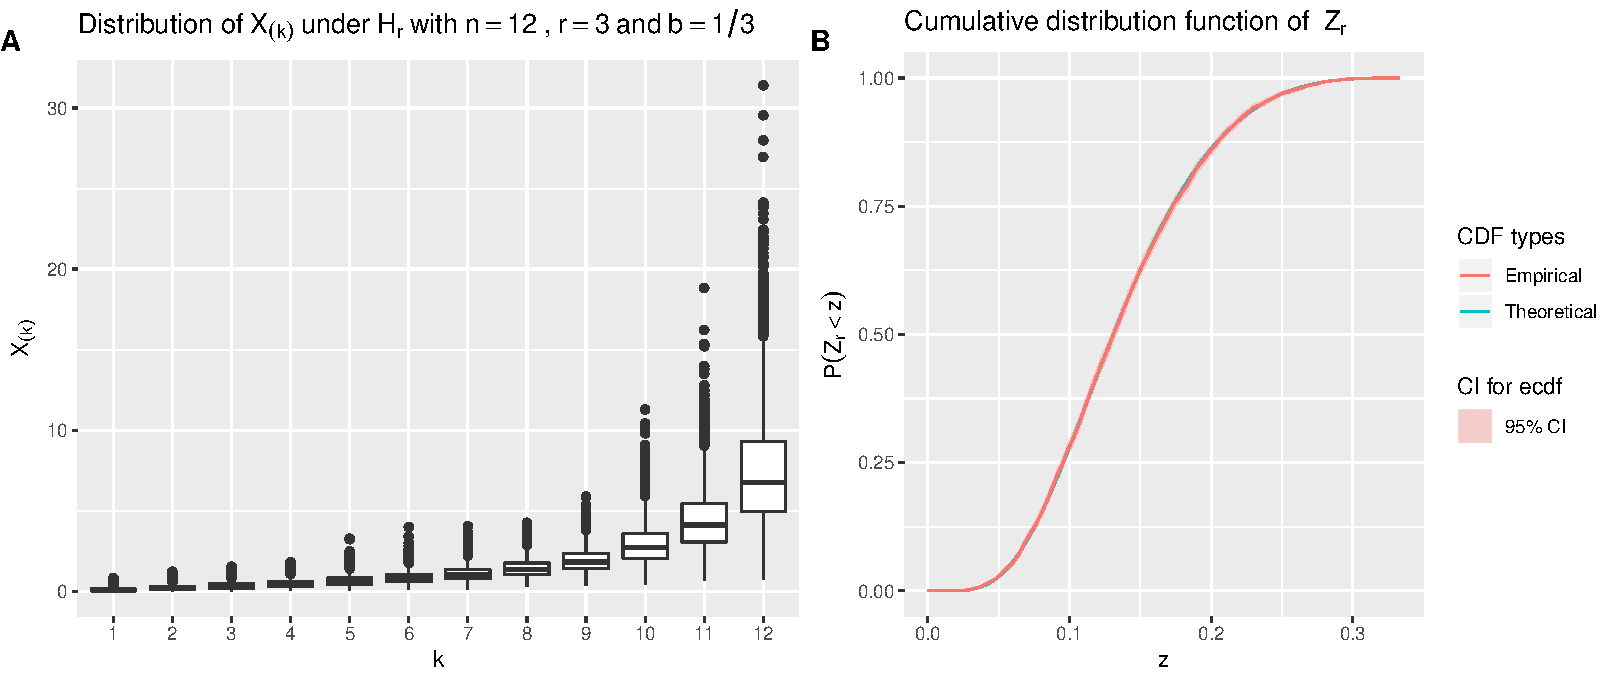
\includegraphics[scale = 0.6]{plot_1.pdf}
    \caption{Distribution of $Z_r$ under $H_r$ with $n =12, r =3, b = 1/3$.}
    {\label{Figure: cdf of Zr}
        \par {\small \begin{itemize}
            \item[A] The box plot of order statistics of the exponential slippage sample generated \\
            \item[B] Empirical distribution function and the theoretical distribution function derived in Theorem \ref{thm: distribution of Z_r}
        \end{itemize}
    }}
\end{figure}

\begin{figure}[hbtp]
    \centering
    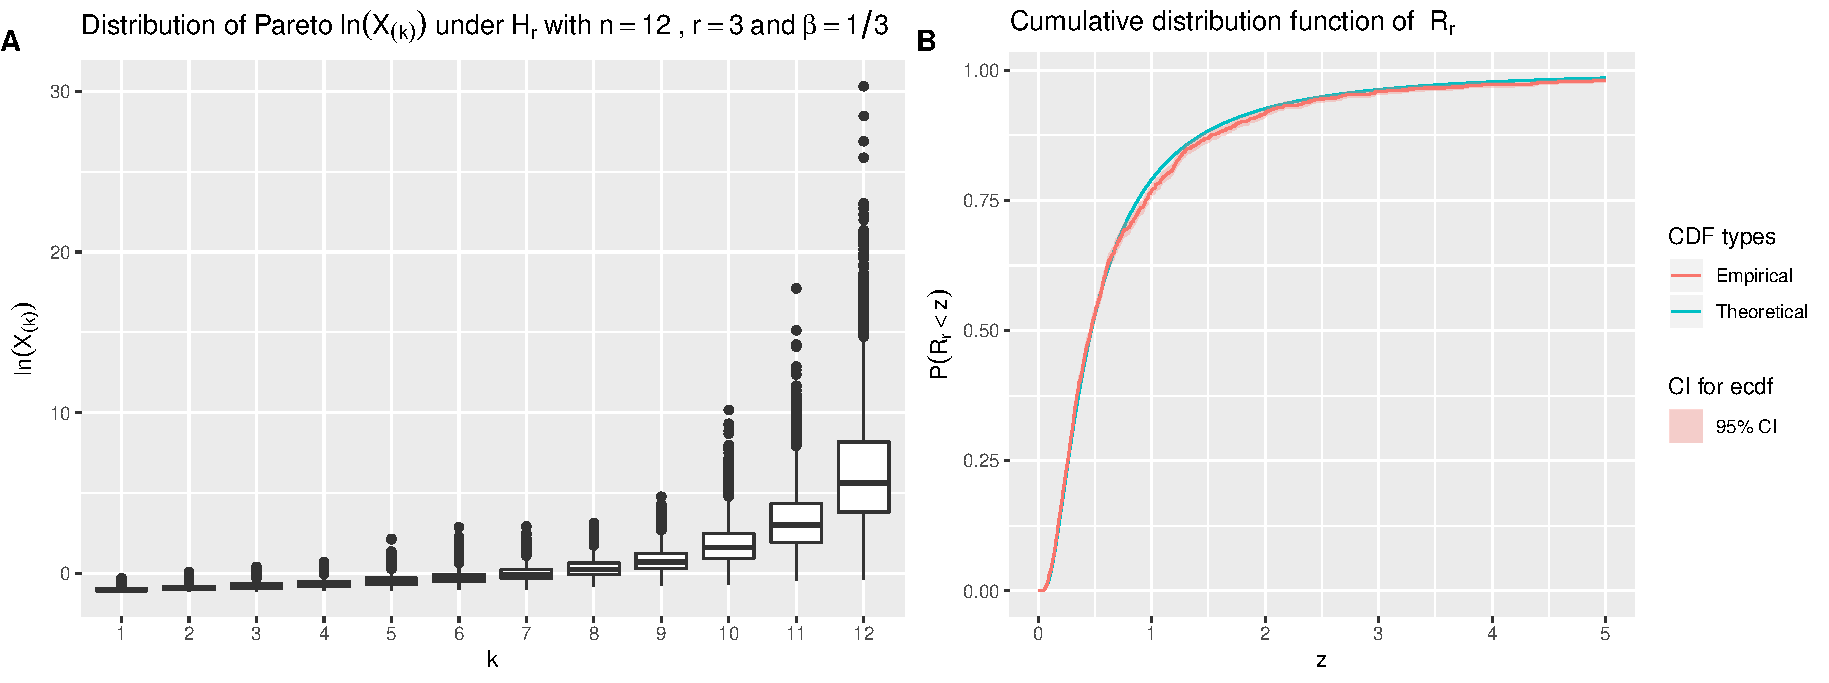
\includegraphics[scale = 0.6]{plot_2.pdf}
    \caption{Distribution of $\tilde R_r$ under $H_r$ with $n =12, r =3, \beta = 1/3$.}
    {\label{Figure: cdf of Rk}
        \par {\small
        \begin{itemize}
            \item[A] The box plot of order statistics of the logarithm of the Pareto samples generated \\
            \item[B] Empirical distribution function and the theoretical distribution function derived in Theorem \ref{thm: distribution of R_r}
        \end{itemize}
    }}
\end{figure}

\section{Performance of Test Statistics Under $H_0$}

Here, we examine the performance of the statistics $Z_r$ and $\tilde R_r$ under $H_0$. In particular, we examine the distribution of $p$-values of the test and
verify that the type-I error has been properly controlled.
In our study, we compared $Z_r$ with Dixon statistic $D_r$ and $\tilde D_r$ for
power comparison based on $5000$ samples, but we did not obtain the exact distribution of $D_r$. So, it is not necessary or possible
to check the type-I error rate of $D_r$ or $\tilde D_r$, since the critical value and distribution of $D_r$ and $\tilde D_r$ are estimated with simulation.
The distribution of the test statistics and empirical $p$-values for $Z_r$ are summarized in Figure \ref{Figure: test stats dis of exp case}.
Since we are considering the upper slippage alternative, the $p$-value is defined to be $\P{Z_r < z \mid H_0}$ for any observed sample statistic $z$.

As can be seen from Panel B of Figure \ref{Figure: test stats dis of exp case}, the empirical distribution of $p$-values is seen to be similar to the
random samples of standard uniform distribution, which is the expected result. We fix the type-I error rate to be $\alpha = 0.05$, and use empirical
$p$-values to estimate the actual type-I error rate by
\[ 
    \hat \alpha = \sumi{B} \frac{1}{B} \I{p_i < 0.05}
\]   
which was found to be $\hat \alpha = 0.0522$, which is also acceptable.

We performed the exact the same procedure to examine the distribution of $\tilde R_r$ for the slippage samples. Since the distribution of the test statistic
$\tilde R_r$ is right skewed, the histogram in Panel A is for the sample of $\tilde R_r$ after the logarithm transformation. The panel B of
the figure shows no contradiction to that empirical $p$-values follow uniform distribution, which is also acceptable.
With the same method, we found the estimated type-I error rate to be $\hat \alpha = 0.048$, which is also close.

    
    \begin{figure}[hbtp]
    \centering
    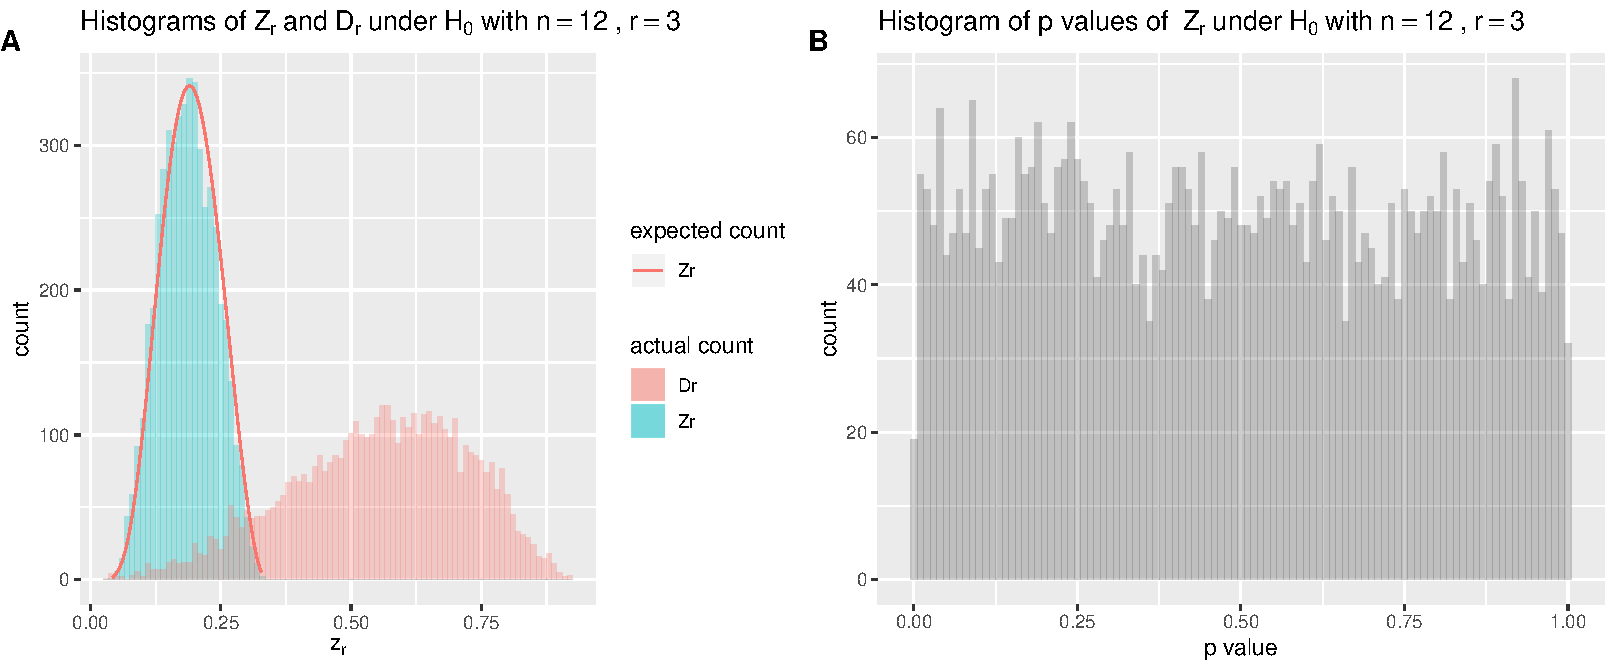
\includegraphics[scale = 0.6]{plot_3.pdf}
    \caption{Distributions of the test statistics $D_r$ and $Z_r$ under $H_r$ with $n =12, r =3, b = 1/3$.}
    {\label{Figure: test stats dis of exp case}
    \par {\small
        \begin{itemize}
            \item[A] The histogram of $Z_r$ and $D_r$; the expected count number of $Z_r$ is estimated with the density of $Z_r$ given in Theorem \ref{thm: distribution of Z_r} \\
            \item[B] The distribution of empirical $p$ values, where each empirical value $p_i$ is defined to be $\P{Z_r(z_i) < z_{r,\alpha} \mid H_0}$, where $z_i$ are the samples generated under $H_r$.
        \end{itemize}
        }}
\end{figure}

\begin{figure}[hbtp]
    \centering
    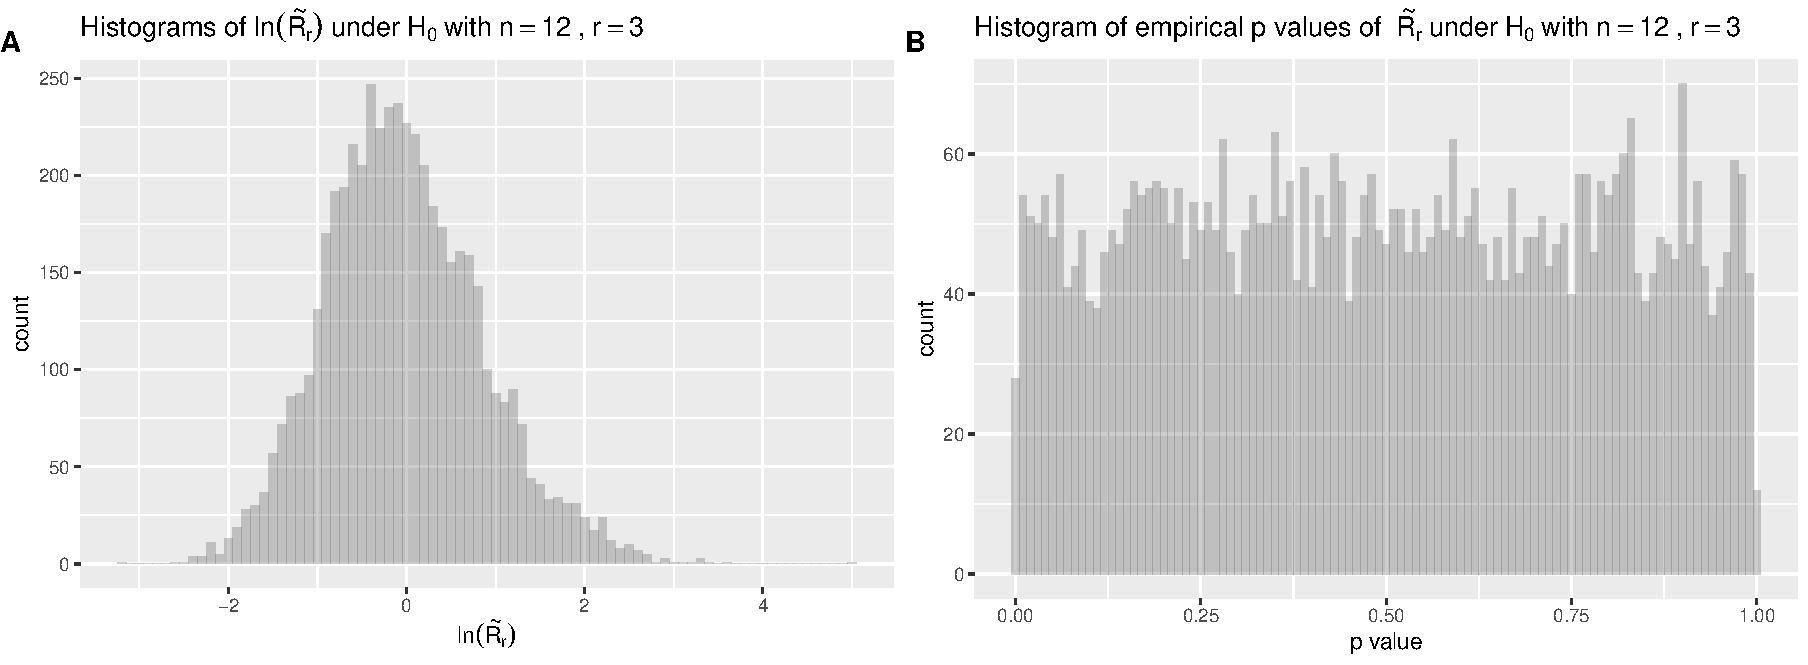
\includegraphics[scale = 0.6]{plot_4.pdf}
    \caption{Distributions of the test statistic of $\ln( \tilde R_r)$ under $H_r$ with $n =12, r =3, b = 1/3$.}
    {\label{Figure: test stats dis of exp case}
    \par {\small
    \begin{itemize}
        \item[A] The histogram of $\ln( \tilde R_r)$
        \item[B] The distribution of empirical $p$ values, where each empirical value $p_i$ is defined to be $\P{\tilde R_r(z_i) < r_{k,\alpha} \mid H_0}$, where $z_i$ are the samples generated under $H_r$.
        \end{itemize}
        }}
    \end{figure}

    \subsection{Critical Values}
    
Since there are mistakes in the derivations of distributions in \cite{zerbet2003new} and \cite{jabbari2019detecting}, here we give tables of the critical values
of $Z_r$ and $D_r$ for testing upper outliers with significance level $1-\alpha$ with $\alpha =0.05$. The critical values for $\tilde R_r$ and $Z_r$ are obtained by finding the
root of $F(x) = \alpha$ for $x$ with bisection method, where $F$ is the distribution functions derived in Theorem \ref{thm: distribution of Z_r} and
Theorem \ref{thm: distribution of R_r}. The critical value for the Dixon statistic was obtained with nonparametric bootstrap method introduced in Section \ref{sec: bootstrap},
and the estimation bias has been taken account to by \eqref{eqn: boot bias}. A table of standard error of the obtained estimates is calculated by \eqref{eqn: boot var} and presented in Table \ref{table: Dr standard error}. As can
be seen from Table\ref{table: Dr standard error}, the critical values we obtained are accurate to three decimal places, and this agrees with the result given in \cite{zerbet2003new}.



\begin{table}[hbtp]
    \centering
    \caption{The critical values of $Z_r$ with $\alpha = 0.05$} \label{table: Zr critical values}
    \begin{tabular}{*{7}{c}}
        \toprule
        \multirow{2}{*}{$n$} & \multicolumn{6}{c}{$r$} \\
        \cline{2-7} 
        & 1 & 2 & 3 & 4 & 5 & 6 \\
        \midrule
        6 & 0.2179255 & 0.07271396 & 0.02257252 & 0.002554801 &           &           \\
        7 & 0.2541362 & 0.09761256 & 0.04158413 & 0.014258365 & 0.001703935 &           \\
        8 & 0.2827005 & 0.11738195 & 0.05767611 & 0.027187769 & 0.009843320 & 0.001217544 \\
        9 & 0.3059432 & 0.13338088 & 0.07094024 & 0.038625121 & 0.019246229 & 0.007211060 \\
        10 & 0.3253324 & 0.14660659 & 0.08194491 & 0.048345371 & 0.027852283 & 0.014371925 \\
        11 & 0.3418340 & 0.15775129 & 0.09119986 & 0.056587249 & 0.035351931 & 0.021105592 \\
        12 & 0.3561090 & 0.16729823 & 0.09909488 & 0.063629961 & 0.041830932 & 0.027096803 \\
        \bottomrule 
    \end{tabular}
\end{table}


\begin{table}[hbtp]
    \centering
    \caption{The estimated critical values of $D_r$ for $\alpha = 0.05$ with Monte Carlo method} \label{table: Dr critical values}
    \begin{tabular}{*{7}{c}}
        \toprule
        \multirow{2}{*}{$n$} & \multicolumn{6}{c}{$r$} \\
        \cline{2-7} 
                    & 1 & 2 & 3 & 4 & 5 & 6 \\
        \midrule
        6 & 0.7451293 & 0.8613298 & 0.9295339 & 0.9721648 &          &         \\
        7 & 0.7174043 & 0.8333060 & 0.8997864 & 0.9454283 & 0.9782023 &         \\
        8 & 0.6937633 & 0.8084582 & 0.8758362 & 0.9217053 & 0.9569222 & 0.9819938 \\
        9 & 0.6748915 & 0.7878169 & 0.8512355 & 0.9002023 & 0.9363351 & 0.9643261 \\
        10 & 0.6572173 & 0.7696995 & 0.8354201 & 0.8819363 & 0.9175486 & 0.9458965 \\
        11 & 0.6438796 & 0.7539956 & 0.8176284 & 0.8643931 & 0.9012357 & 0.9296735 \\
       12 & 0.6313994 & 0.7392545 & 0.8037565 & 0.8488094 & 0.8850763 & 0.9146531 \\
       \bottomrule 
    \end{tabular}
\end{table}

\begin{table}[hbtp]
    \centering
    \caption{The estimated critical values of $ R_r$ for $\alpha = 0.05$} \label{table: Rk critical values}
    \begin{tabular}{*{7}{c}}
        \toprule
        \multirow{2}{*}{$n$} & \multicolumn{6}{c}{$r$} \\
        \cline{2-7} 
        & 1 & 2 & 3 & 4 & 5 & 6 \\
        \midrule
        6 & 0.1501963 & 0.04632501 & 0.00565403 &             &          \\ 
        7 & 0.2092279 & 0.08857200 & 0.03191082 & 0.004138095 &          \\ 
        8 & 0.2607984 & 0.12798613 & 0.06301878 & 0.024141817 & 0.003232332 \\
        9 & 0.3062225 & 0.16364416 & 0.09308207 & 0.048699504 & 0.019287215 \\
       10 & 0.3466706 & 0.19582426 & 0.12095287 & 0.073033005 & 0.039504091 \\
       11 & 0.3830610 & 0.22499710 & 0.14656179 & 0.096008036 & 0.059916655 \\
       12 & 0.4160997 & 0.25160775 & 0.17010112 & 0.117415965 & 0.079466899 \\
       \bottomrule 
    \end{tabular}
\end{table}



\begin{table}
        \centering
        \caption{The standard errors of the estimate of critical values of $D_r$ for $\alpha = 0.05$} \label{table: Dr standard error}
        \begin{tabular}{*{7}{c}}
                \toprule
                \multirow{2}{*}{$n$} & \multicolumn{6}{c}{$r$} \\
                                        \cline{2-7} 
                            & 1 & 2 & 3 & 4 & 5 & 6 \\
                \midrule
                6 & 0.0003654004 & 0.0006721107 & 0.0004517287 & 0.0002250101 &              &             \\
                7 & 0.0003930877 & 0.0007751294 & 0.0005556101 & 0.0003343549 & 0.0001549828  &             \\
                8 & 0.0004040385 & 0.0008054345 & 0.0005574572 & 0.0003964377 & 0.0002388118  & 0.0001299860 \\
                9 & 0.0003597688 & 0.0008568465 & 0.0006336613 & 0.0004514928 & 0.0003180044  & 0.0002395700 \\
               10 & 0.0003644383 & 0.0008356480 & 0.0006315783 & 0.0004870168 & 0.0004525706  & 0.0002701931 \\
       11 & 0.0003900676 & 0.0008706266 & 0.0007761038 & 0.0005363027 & 0.0004374640  & 0.0003245950 \\
       12 & 0.0003680189 & 0.0008683104 & 0.0007025402 & 0.0005738111 & 0.0004305760  & 0.0003728830 \\
  \bottomrule 
    \end{tabular}
\end{table}

\newpage
\section{Power Estimation}
With the critical values obtained, we can now compare the power values of the test statistics. Here we compare the power of $Z_r$ and $\tilde R_r$
with the Dixon statistic and the result is given in Figure \ref{Figure: powers}. The power of $D_r$ are given by
$\gamma_{Dr}(b_0) = \P{ D_r \leqslant d_{r,1-\alpha}\mid b = b_0}$,
where $d_{r,1-\alpha}$ is the quantile of $R_r$ under $H_0$, since clearly $D_r$ will tend
to $0$ as the parameter $b$ tends to $0$. Similarly, one can show that $R_r$ and $Z_r$ will tend to $0$
as $b$ tends to $0$, hence their power are given by $\gamma_{Rr}(b_0) = \P{ Z_r > z_{r,1-\alpha}\mid b = b_0}$
and $\gamma_{Z_r}(b_0) = \P{ R_r > z_{r,1-\alpha}\mid b = b_0}$.

The power of $\tilde R_r$ and $Z_r$ can be obtained directly since we have 
derived their distributions; the power of Dixon statistic are obtained by Monte Carlo method, where each data point is calculated
with $5000$ simulated samples. It follows from Corollary \ref{cor: distribution of log Pareto OS under Hr} that the test
statistics we have investigated in this study, $Z_r$, $R_r$ and Dixon statistic, can be used to test the slippage alternative
for both exponential and Pareto samples, and we have summarized their power in Figure \ref{Figure: powers}. As
can be seen from the figure, the Dixon statistic is superior to other two test statistics in terms of power.

Jabbari Nooghabi also suggested the following test statistic \cite{jabbari2019detecting} to test $H_r$ for Pareto samples:
\[ 
    T = \frac{Y_{n-r+1} - Y_{(n-r)}}{\hat Y_{(n-r+1)} - Y_{(n-r)}},
\]
where $\hat Y_{(n-r+1)}$ is the BLU estimator of $Y_{(n-r+1)}$ proposed in \cite{kaminsky1975best}, and $Y$ has the two-parameter
exponential distribution such that $X = e^Y$ will yield the desired Pareto random variables. However, since the sample size $n$ we have
considered are relatively small and $\hat Y_{(n-r+1)}$ is justified with asymptotic theory, it is not appropriate to consider here in this study.

\begin{figure}[htbp]
    {\centering
    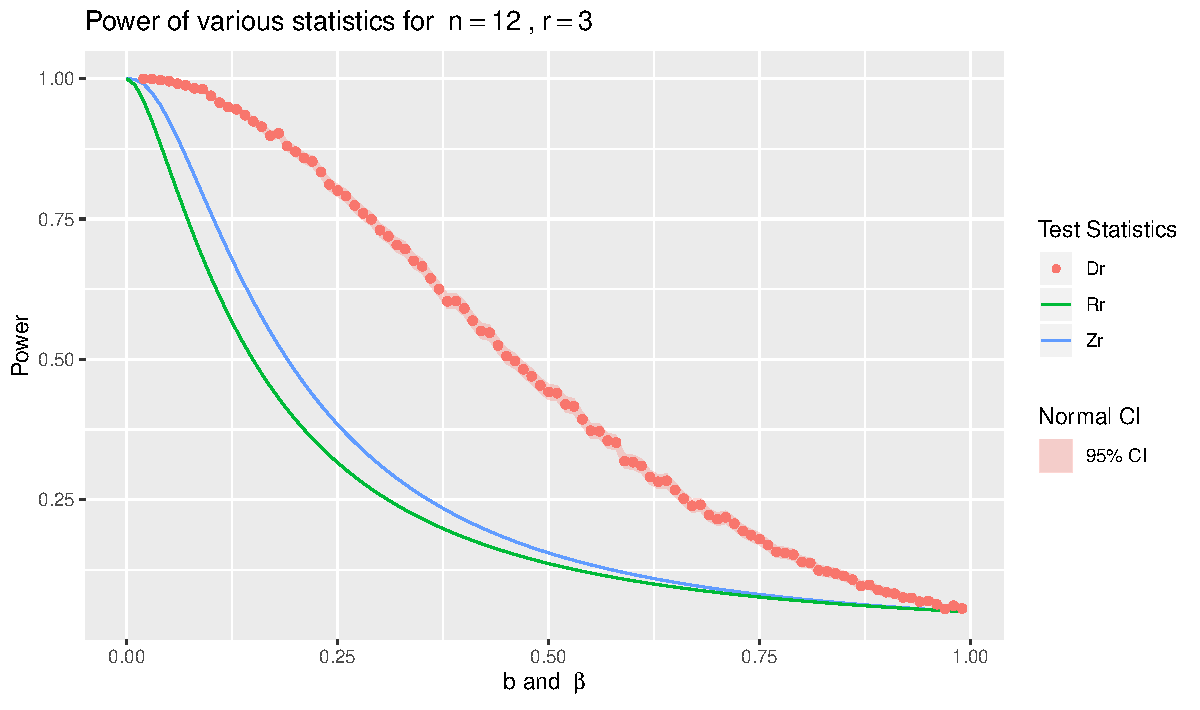
\includegraphics[scale = 0.55]{plot_5.pdf}
    \caption{\label{Figure: powers}Power comparison for various test statistics with $n =12, r =3, b = 1/3$.}}
\end{figure}
\section{Numerical Example}

Here we present a illustrative example based on a real-life dataset to evaluate the performance of the tests. We considered Haberman's survival dataset \cite{lim1999haberman},
which comes from a study that was conducted between 1958 and 1970 at the University of Chicago's Billings Hospital on the survival of patients who had undergone surgery for breast cancer.
Haberman's survival dataset records the number of positive axillary nodes detected for $305$ patients and whether they are still alive 5 years after the surgery, as depicted in Figure \ref{Figure: cancer}.
According to the literature, number of positive axillary nodes are postively correlated to the prognosis of breast cancer \cite{fisher1983relation}, so the distribution of
detected positive axillary nodes of patients are expected to be different between people who survived and thoese did not.
In fact, according to Haberman's survival dataset, the average detected number for survived and passed away patients are found to be $2.80$ and $7.46$, respectively. 

As Figure \ref{Figure: cancer} suggests, the distribution of detected positive axillary nodes
can be modeled by exponential distribution, with mean different based on the survival status of patients. To examine the performance of the test,
we randomly select $12$ patients at random. Since $81$ out of $305$ patient passed away $5$ years after the treatment, we can assume $3$ out of $12$ patient we have drawn are those passed away. 
So, we should take $n = 12$ and $r =3$ when construting the slippage alternative hypothesis.

To examine the power of the tests, with each drawn sample $\mathbf x_0$, we then calculate the test statistics $R_{3}(\mathbf x_0)$, $D_{3}(\mathbf x_0)$ and $Z_{3}(\mathbf x_0)$.
By checking Table \ref{table: Dr critical values}, Table \ref{table: Rk critical values} and Table \ref{table: Zr critical values}, we will reject $H_0$
with $D_r$ if $D_{3}(\mathbf x_0) > 0.80375$, with $R_r$ if  $R_{3}(\mathbf x_0) < 0.17010$ and with $Z_r$ if $Z_3(\mathbf x_0) < 0.09909$.

We have taken $1000$ random samples from Haberman's survival dataset and conducted a hypothesis testing with each drawn sample as described. We found that, the hypothesis testing
procedures based on $D_r$, $Z_r$ and $R_r$ have successfully reject $H_0$ for $475$ and $454$ and $285$ times among $1000$ trials conducted, respectively.
So, the empirical power comparison based on this real dataset is consistent with the power estimation given in Figure \ref{Figure: powers}.

\begin{figure}[hbtp]
    {\centering
    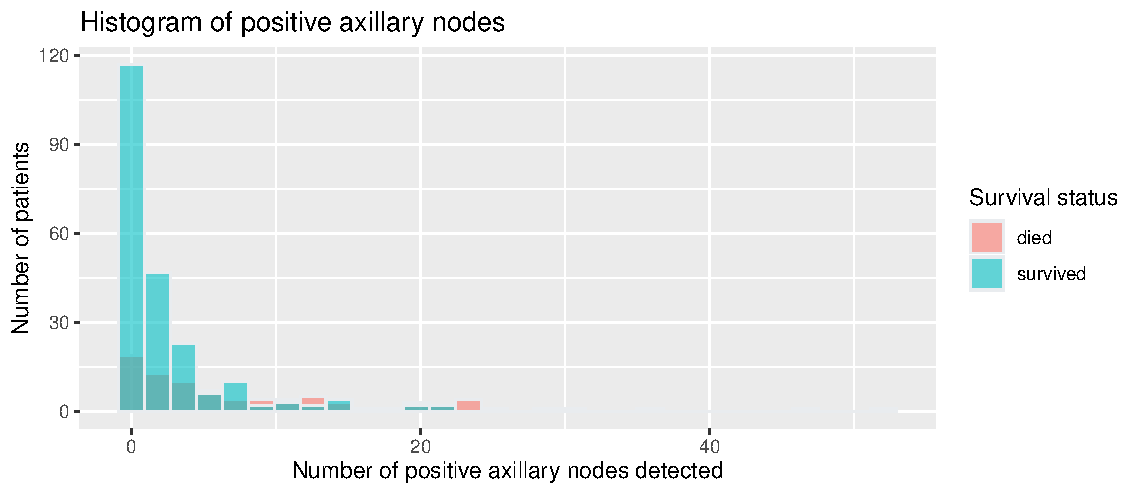
\includegraphics[scale = 0.6]{plot_cancer.pdf}
    \caption{\label{Figure: cancer}Histogram of number positive axillary nodes detected by the survival status of the patients}}
\end{figure}



\section{Discussions and Conclusions}

In this study, we have characterized the distribution of order statistics under smooth monotone transformation in Theorem \ref{thm: monoton transform of order stats}.
Then we have given methods that transform the test for slippage alternative $H_r$ for exponential samples to the Pareto case.
Next, we have investigated some test statistics proposed by Zerbet and Nikulin \cite{zerbet2003new} and Jabbari Nooghabi \cite{jabbari2019detecting} and derived their distributions under $H_r$.
Besides correcting mistakes in the derivation in \cite{jabbari2019detecting}, the usage of Corollary \ref{cor: distribution of order stats} significantly simplified the
proof for the distribution of $\tilde Z_r$. Finally, we proposed have a modified Dixon statistic $\tilde D_r$ that can be used for testing the slippage alternative for
the Pareto case.

Through simulation study, we have given a corrected usable table for critical values for all test statistics investigated and have conducted a power comparison for the case
with sample size $n = 12$, contamination number $r =3$ for various choices of parameter $b$. The simulation study suggests that the Dixon statistics has the best
performance in terms of power. However, we did not obtain the theoretical distribution of Dixon statistic. Moreover, the test statistic $Z_r$ and $R_r$ did
controlled the type-I error rate under the null hypothesis.

Although there are some mistakes in two papers by Zerbet and Nikulin \cite{zerbet2003new} and Jabbari Nooghabi \cite{jabbari2019detecting}, they do
shed some light on the treatment on testing slippage alternative hypothesis. The novelty of the work by Zerbet and Nikulin lies in the fact that they provide a
method to derive the distribution of some function of order statistics with the use of characteristic function. In particular, they used Lemma \ref{Lemma: order statistic transformation}
to transform the problem of derivation the joint distribution of order statistics into that of finding the distribution of independent exponential random variables, which reduces the
complexity of the task. Although not explicitly stating the result as we have done, Jabbari Nooghabi used the relationship between exponential and Pareto distributions to
define some test statistics that can be used to test the slippage alternative for the case of Pareto samples, his method motivated us to define the modified Dixon statistic
$\tilde D_r$.

For future work, one could use the method introduced in \cite{zerbet2003new}
to obtain the distribution of $D_r$. Another challenge is, how to determine whether it is appropriate to
assume slippage alternative hypothesis. As we have pointed out in Figure \ref{Figure: efficiency}, the slippage alternative
is appropriate only if the number of contanminants is relatively small and mean difference between the contaminated samples
and the samples assumed coming from null hypothesis is large enough.


\bibliographystyle{unsrt}
\bibliography{short_summary}
\end{document}